\documentclass[numbering=fraction]{beamer}

\usepackage[utf8]{inputenc}
\usepackage{blindtext}
\usetheme{Malmoe}

\setbeamertemplate{navigation symbols}{}


\usecolortheme{dove}
\useinnertheme{rectangles}
\setbeamertemplate{footline}{}

%Define colors
\definecolor{wuppergreen}{RGB}{100, 100, 100}
\definecolor{background}{RGB}{255,255,255}
\usefonttheme{serif}
\usepackage{multicol}
%Adding logo to title page
\titlegraphic{
\includegraphics[width=1cm]{ENS.png}}

%Adjust color theme
\setbeamercolor{title separator}{fg=wuppergreen}
\setbeamercolor{footline}{fg=gray}
\setbeamercolor{progress bar}{fg=blue}
\setbeamerfont{frametitle}{size=\small,series=\scshape}
\setbeamerfont{itemize/enumerate body}{size=\small}
%Adding footer

%Set parameters for title page

\title{Shallow water equations \& Poincaré waves}\author{Andrea \textsc{Combette}}
\institute{ENS ULM}
\date{\today{}}


\begin{document}
\begin{frame}
    \titlepage
\end{frame}
\section{Introduction}
\begin{frame}
    \frametitle{Shallow water equations \& Poincaré waves}
    \begin{minipage}{0.6\linewidth}
        \begin{itemize}
            \item fundamental in fluid dynamics
            \item thin fluid layer compared to its horizontal extension
            \item Poincaré waves: frictionless and Coriolis dependent nature
            \item Subsets of solutions : Rossby waves, Kelvin waves, Inertia-gravity waves
        \end{itemize}
    \end{minipage}
    \hfill
    \begin{minipage}{0.38\linewidth}
        \begin{figure}[H]
            \hspace*{-3cm}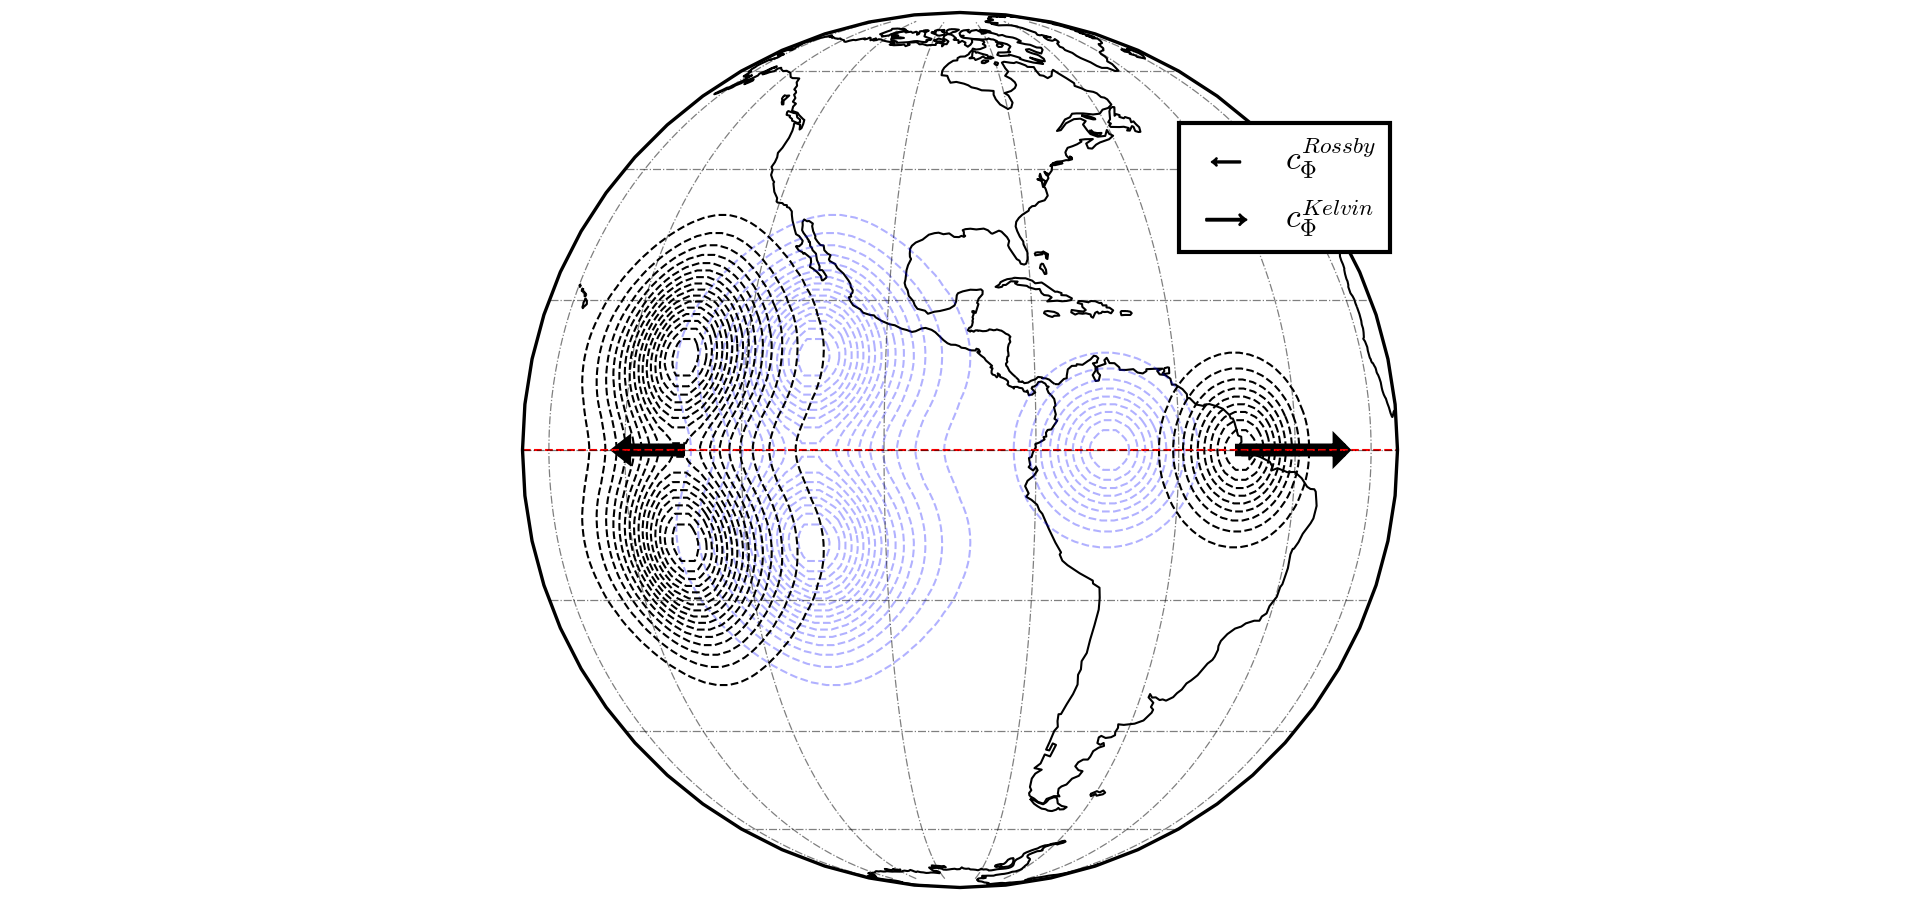
\includegraphics[width=2.5\linewidth]{./figure/earth_view.png}
            \caption{\footnotesize{Earth view of the equatorial domain.}}
            \label{fig:}
        \end{figure}
    \end{minipage}
\end{frame}

\section{Theoretical background}
\subsection{Shallow water equations}
\begin{frame}
    From first order perturbation we got :
    \frametitle{Differential equation system}
    \begin{equation} \label{eq:1}
        \begin{cases}
            \partial_t u  - fv = -g \partial_x h \\
            \partial_t v + fu = -g \partial_y h  \\
            \partial_t h + a_0( \partial_x u + \partial_y v) = 0
        \end{cases}
    \end{equation}
    \begin{itemize}
        \item equatorial study to simply the coriolis parameter dependence
        \item Beta plane approximation  : $f = \beta y$
        \item scale dependence of solutions behavior : study of the zonal wave number
    \end{itemize}
\end{frame}
\subsection{Equatorial Study}
\begin{frame}
    \frametitle{Equatorial solutions}
    The equatorial study leads at first order to the following solutions,
    using slow variable : $\xi, \tau$ :
    \begin{equation}
        \label{eq:Rossby}
        \begin{cases}
            v^0(y, \xi, \tau) = \partial_\xi \eta(\xi, \tau) e^{-(1/2)y^2}H_n(y)                                     \\
            u^0(y, \xi, \tau) = \eta(\xi, \tau) [ \frac{H_{n+1}(y)}{2(1-c)} - \frac{nH_{n-1}(y)}{1 +c}]e^{-(1/2)y^2} \\
            h^0(y, \xi, \tau) = \eta(\xi, \tau) [ \frac{H_{n+1}(y)}{2(1-c)} + \frac{nH_{n-1}(y)}{1 +c }]e^{-(1/2)y^2}
        \end{cases}
    \end{equation}
    With $H_n$ the Hermite polynomials and $c = -   \frac{1}{2n + 1}$ the phase velocity of the n-th mode of propagation. And $\eta(\xi, \tau)$ the envelope function, defined by KDV equation solving.
\end{frame}

\begin{frame}
    \frametitle{dispersion relation}
    The dispersion relation can be expressed by the following :
    \begin{equation}
        \label{eq:7}
        \sigma^3 = \sigma [k^2 \epsilon^{-1} + \epsilon^{-1/2}(2n + 1)] + k\epsilon^{-1}
    \end{equation}
    \begin{itemize}
        \item $\sigma$ is the dimensionless frequency, $k$ the zonal wave number, $\epsilon$ is a constant depending on the system parameter.
        \item Third order : 3 solutions
    \end{itemize}
\end{frame}

\begin{frame}
    \frametitle{Rossby wave frequency study}
    \begin{minipage}{.7\linewidth}
        \begin{figure}[H]
            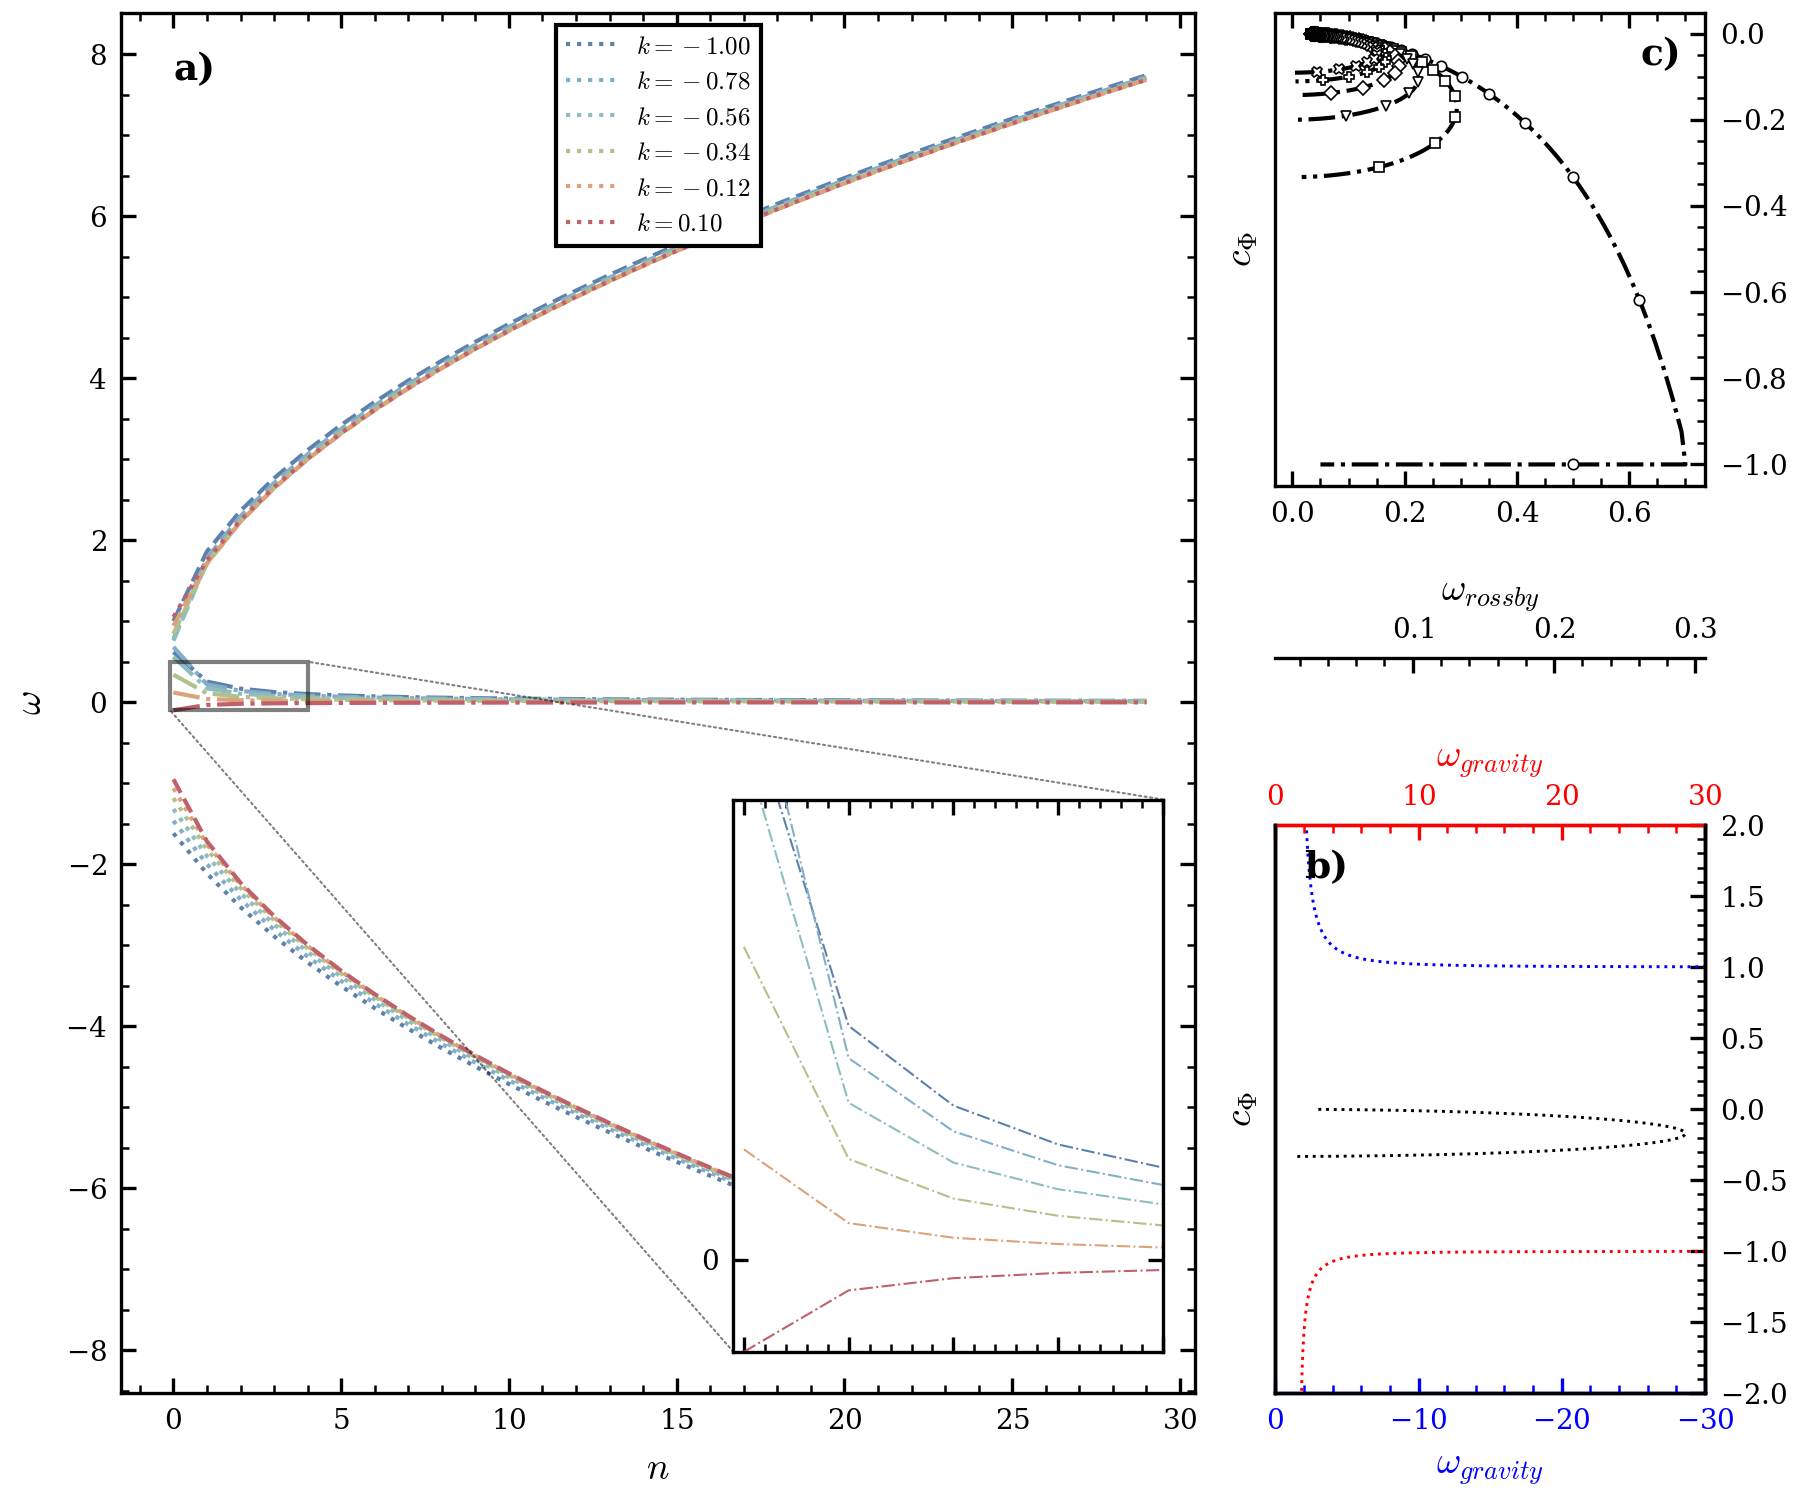
\includegraphics[width=1\linewidth]{./figure/roots.png}
            \label{fig:}
        \end{figure}
    \end{minipage}
    \hfill
    \begin{minipage}{.28\linewidth}
        \begin{itemize}
            \item low mode weakly dispersive
            \item 2 types of wave
            \item $n = 0$ strongly dispersive
        \end{itemize}
    \end{minipage}
\end{frame}

\begin{frame}
    \frametitle{Rossby wave spatial study}
    \begin{minipage}{.7\linewidth}
        \begin{figure}[H]
            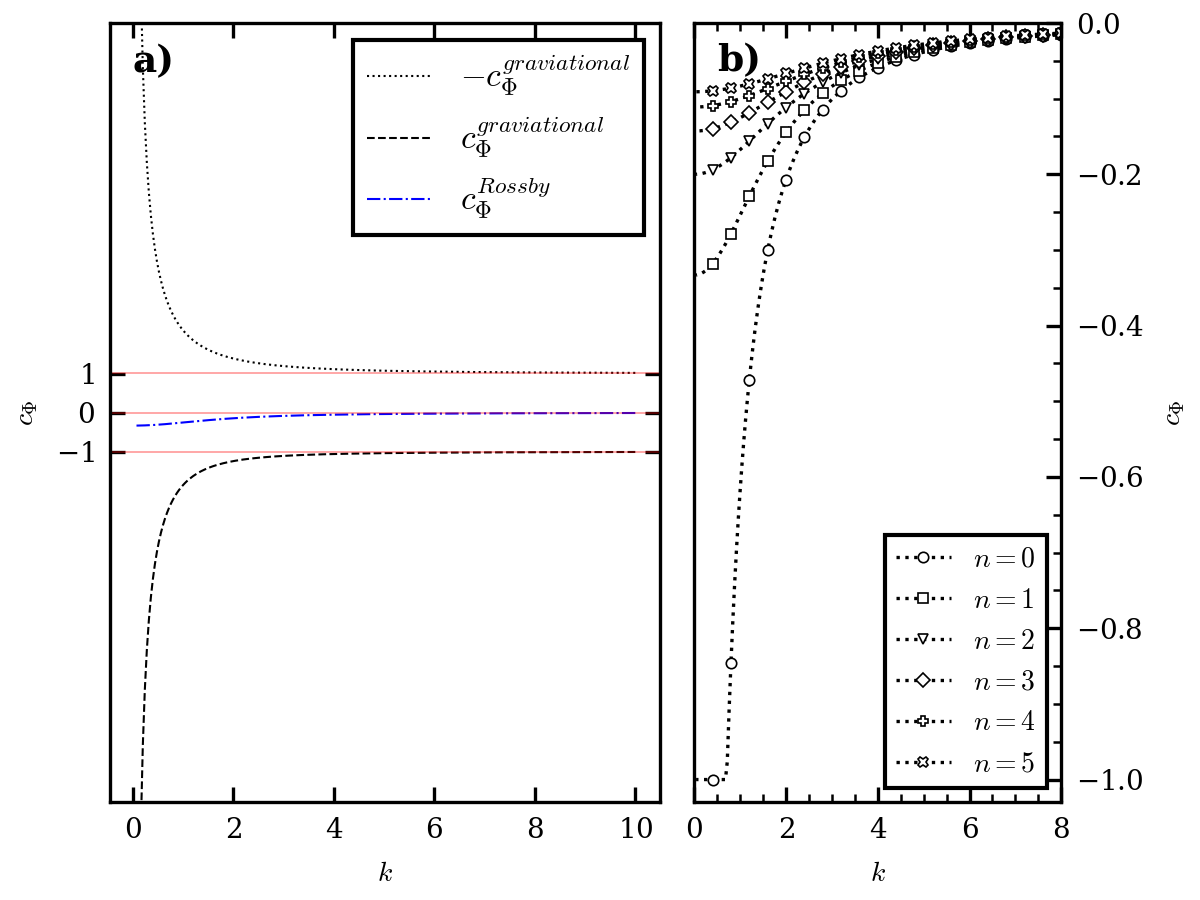
\includegraphics[width=1\linewidth]{./figure/roots_k.png}
            \label{fig:}
        \end{figure}
    \end{minipage}
    \hfill
    \begin{minipage}{.28\linewidth}
        \begin{itemize}
            \item large scale to have weakly dispersive Rossby waves
            \item always westward
        \end{itemize}
    \end{minipage}
\end{frame}

\begin{frame}
    \frametitle{First mode of rossby wave}
    For the first mode we got $c_\Phi = -1/3$ and :
    \begin{equation}
        \label{eq:8}
        \eta(\xi, \tau) = A \text{sech}^2[B(\xi - 0.395B^2\tau)]
    \end{equation}
    \begin{figure}[H]
        \hspace*{-.5cm}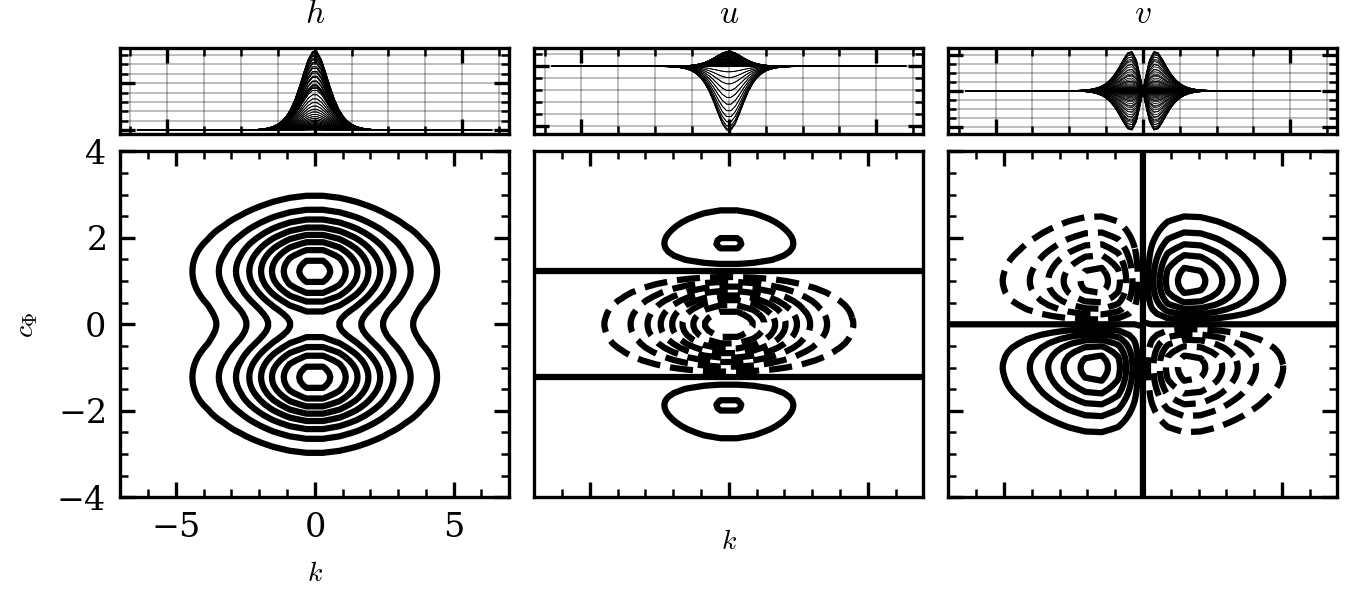
\includegraphics[width=1\linewidth]{./figure/initial_data.png}
    \end{figure}
\end{frame}

\begin{frame}
    \frametitle{Kelvin wave}
    An other type of solution is the Kelvin wave, with $n = -1$ defined by :

    \begin{minipage}{.38\linewidth}
        \begin{equation}
            \begin{cases}
                u(\xi) = U_{-1}e^{-(1/2)\xi^2} \\
                v(\xi) = 0                     \\
                h(\xi) = U_{-1}\frac{\sigma}{k}e^{-(1/2)\xi^2}
            \end{cases}
        \end{equation}
    \end{minipage}
    \hfill
    \begin{minipage}{0.6\linewidth}
        \begin{figure}[H]
            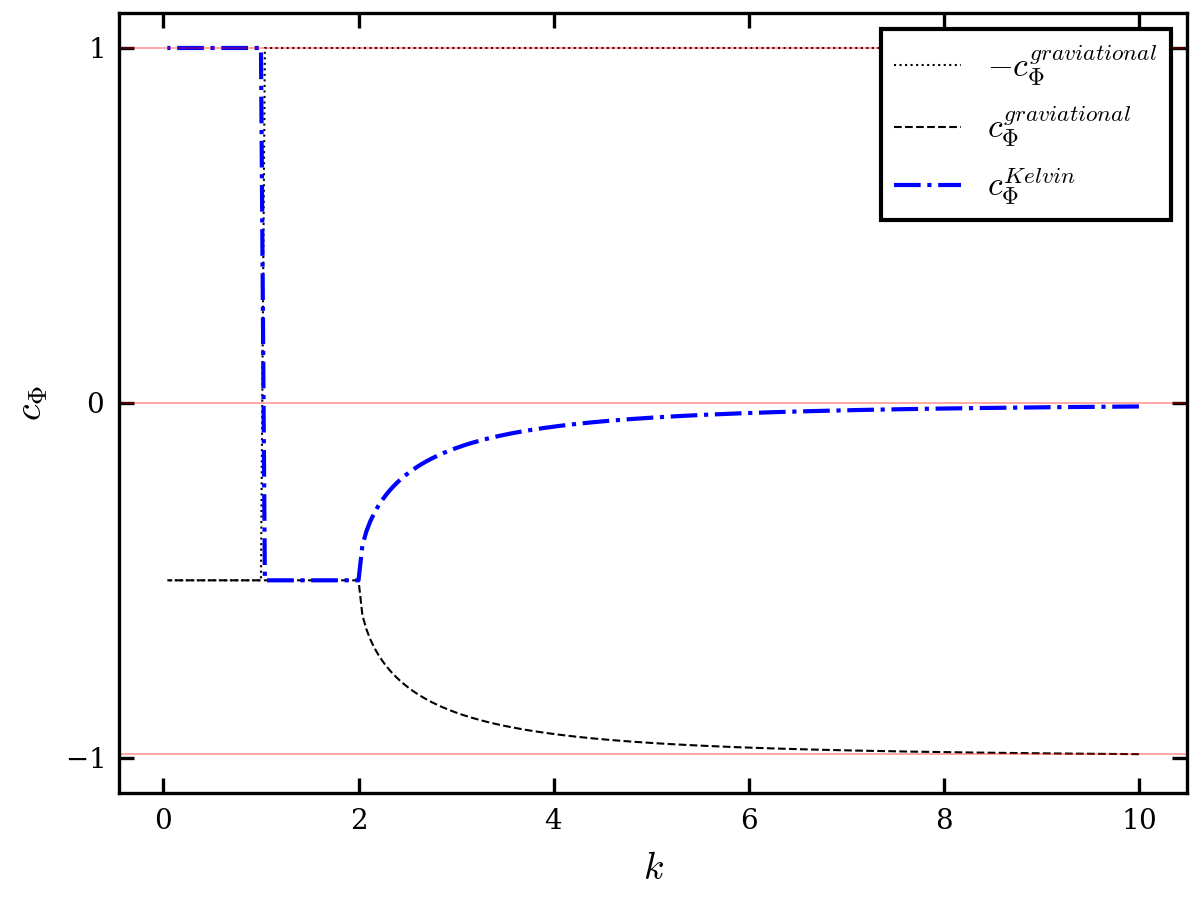
\includegraphics[width=1\linewidth]{./figure/roots_k2.png}
            \label{fig: Kelvin mode}
        \end{figure}
    \end{minipage}
\end{frame}


\section{Numerical implementation}
\begin{frame}
    \frametitle{Numerical implementation}
    \begin{enumerate}
        \item No damping effect
        \item Numerical errors
        \item soliton is a good way to test the scheme
    \end{enumerate}
\end{frame}
\subsection{Integration scheme}
\begin{frame}
    \frametitle{Integration scheme}
    \begin{itemize}
        \item Chebyshev spectral method
        \item domain $[-24, 24] \times [-4, 4]$
        \item To be in the scope of Boyd study
    \end{itemize}
\end{frame}
\subsubsection{Spatial discretization}
\begin{frame}

    \frametitle{Spatial discretization}
    $$x'_{i,j} = (\alpha \cos(\frac{i\pi}{N}), \beta \cos(\frac{j\pi}{N}))$$

    \begin{minipage}{.48\linewidth}
        To be in the following range : $[-\alpha, \alpha] \times [-\beta, \beta]$. Here we will choose $\alpha = 24, \, \beta = 4$
        This gives the following mesh :
    \end{minipage}
    \begin{minipage}{.5\linewidth}
        \begin{figure}[H]
            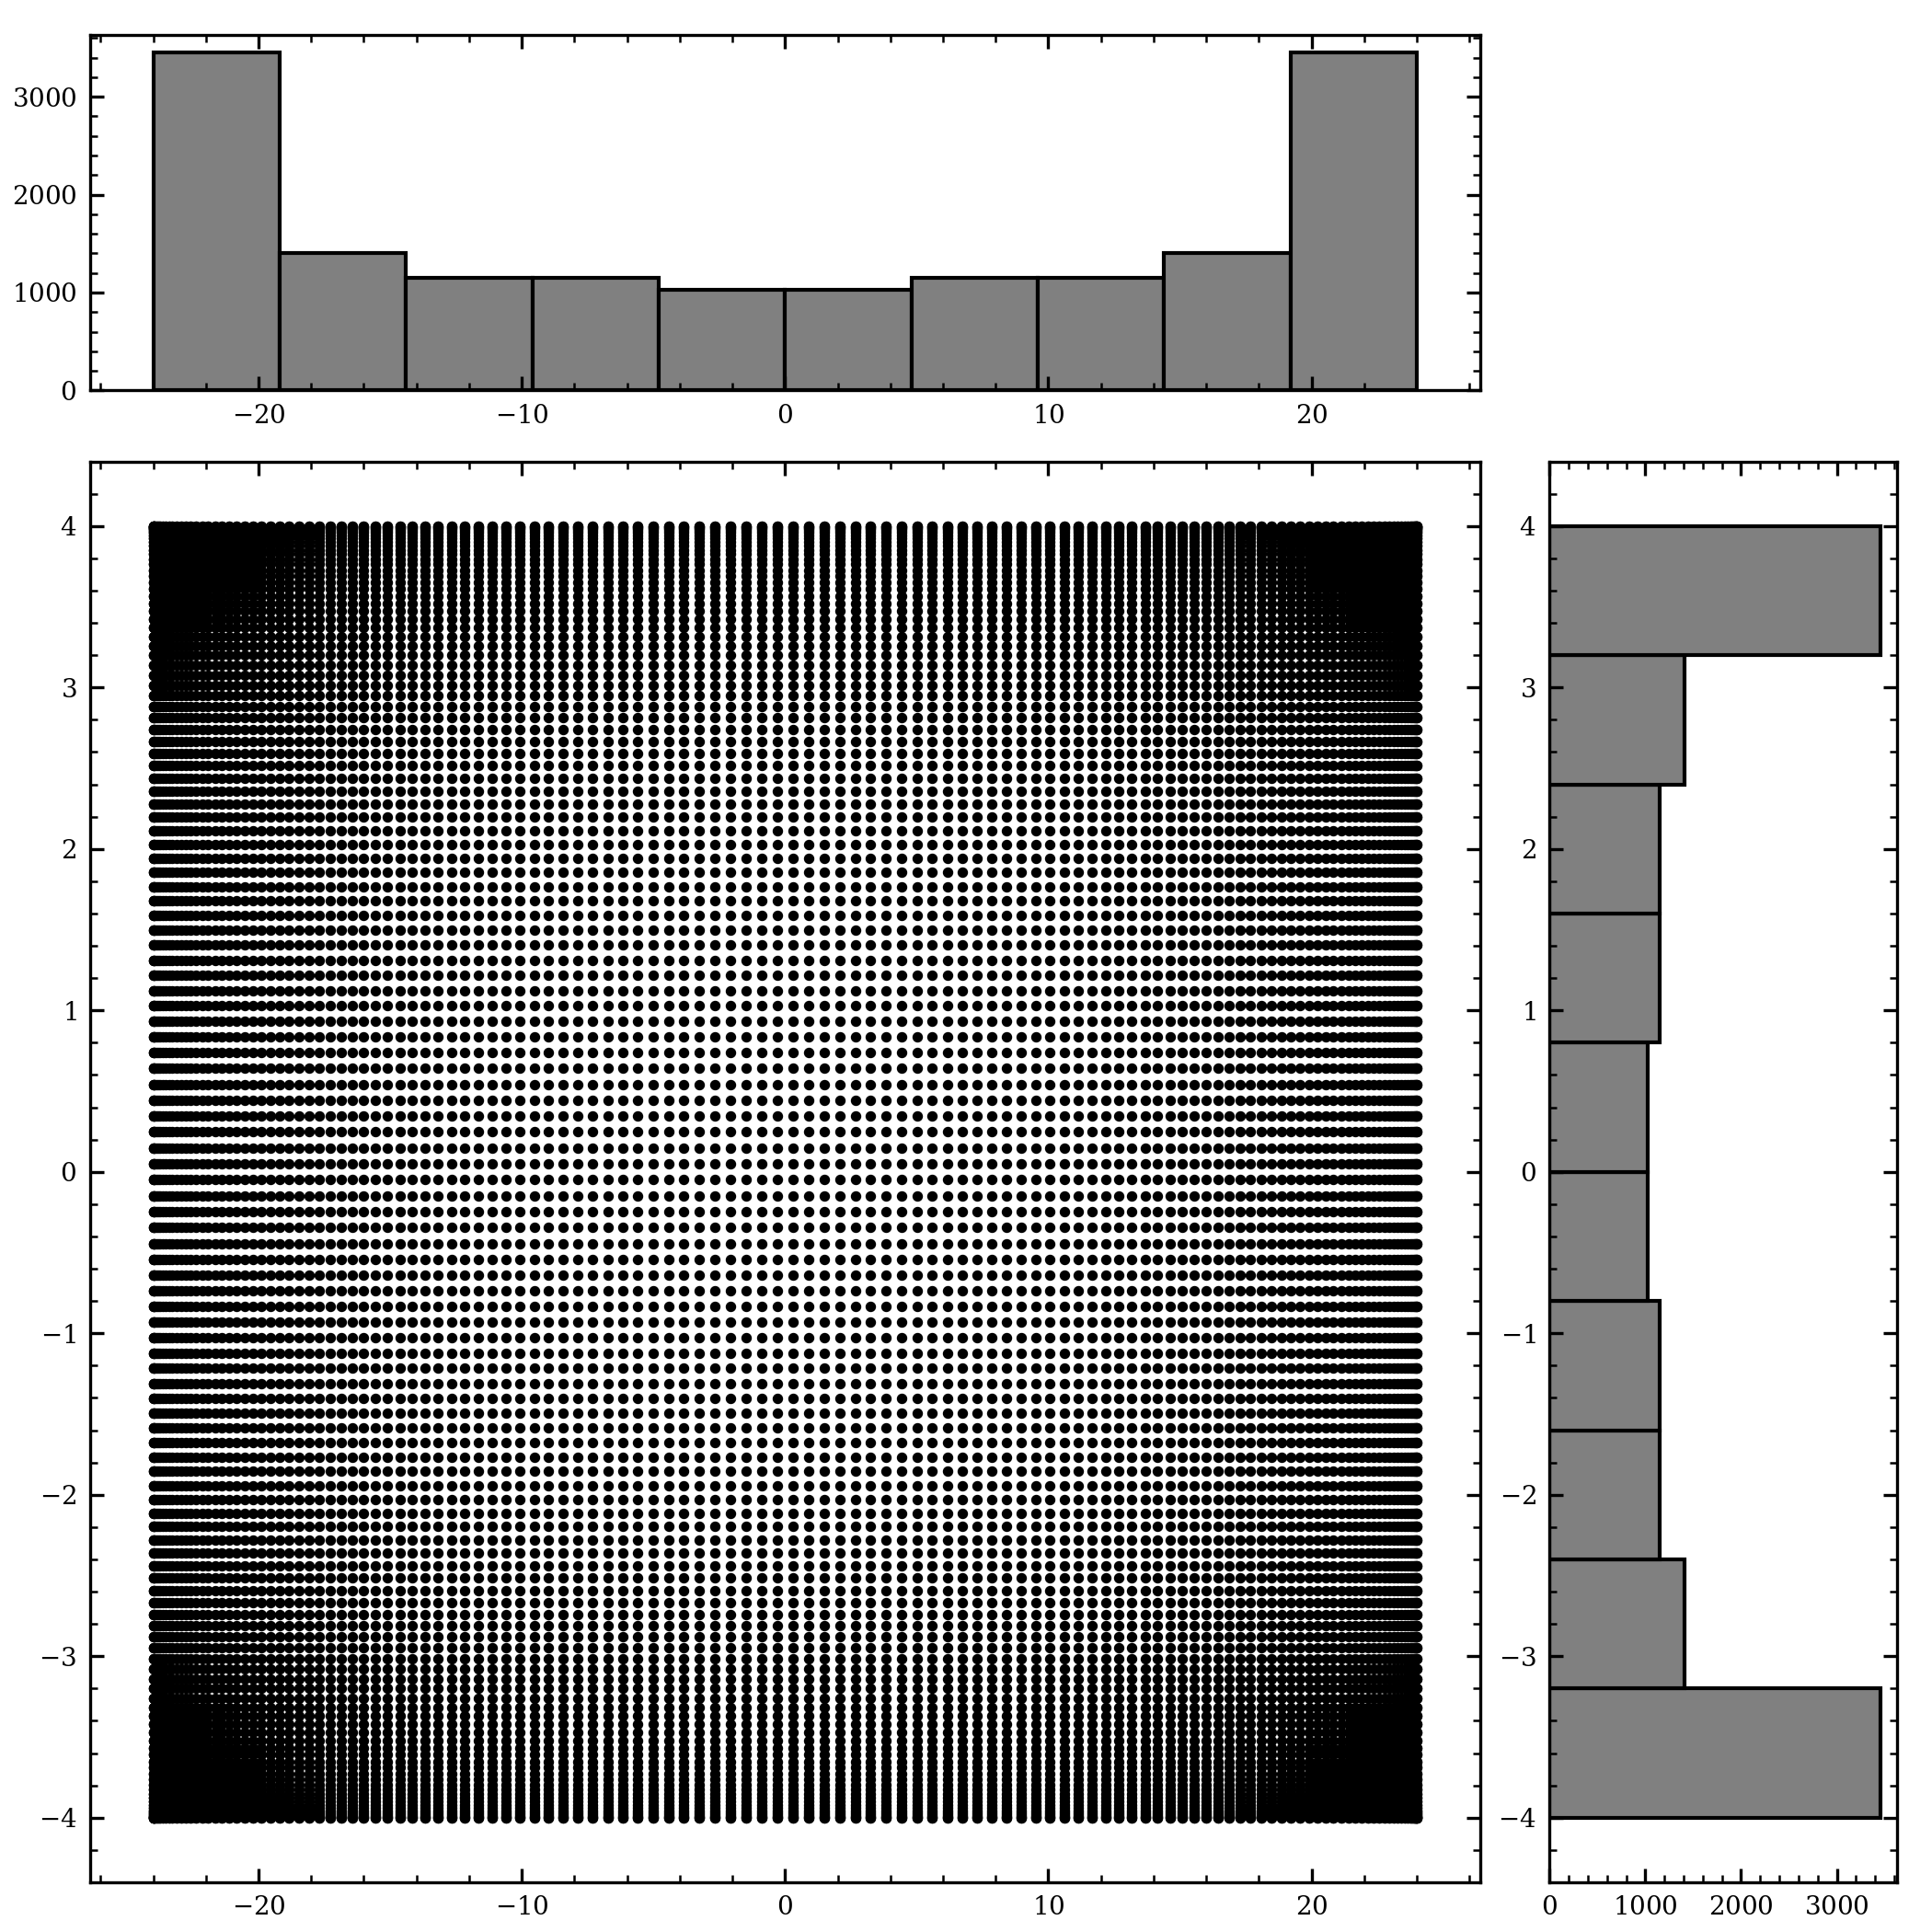
\includegraphics[width=1\linewidth]{./figure/mesh.png}

        \end{figure}
    \end{minipage}
\end{frame}

\subsubsection{Time discretization}
\begin{frame}
    \frametitle{Time discretization}
    \textbf{leap-frog like} method
    $$\partial_t u(t) \approx \frac{u(t + \Delta t) - u(t - \Delta t)}{2\Delta t}$$
    \begin{equation}
        \label{eq:10}
        \begin{cases}
            u^{n+1}  = u^{n-1} + 2\Delta t -g \partial_x h^n + fv^n \\
            v^{n+1}  = v^{n-1} + 2\Delta t -g \partial_y h^n - fu^n \\
            h^{n+1}  = h^{n-1} - 2\Delta t a_0( \partial_x u^n + \partial_y v^n) = 0
        \end{cases}
    \end{equation}
\end{frame}
\subsubsection{CFL Condition}
\begin{frame}
    \textbf{CFL conditions} is strongly impacted by the spectral mesh with irregular spacing
    \frametitle{CFL conditions}
    $$C=\Delta t\left(\sum _{i=1}^{n}{\frac {u_{i}}{\Delta x_{i}}}\right)\leq C_{\max}.$$
    $$C=\Delta t\left(\frac {u_{1}}{\Delta x_{1}}\right)\leq C_{\max }.$$
    $$\Delta_x = 1 - \cos(\frac{1}{N}) \approx \frac{1}{N^2}.$$
    Hence we have the following condition : $\Delta_t \le 3C_{\max} N^{-2}$, we determined $C_{\max} = 5.532$ using many, time and space discretization
\end{frame}

\subsection{Boundary conditions}
\begin{frame}
    \frametitle{Boundary conditions}
    \begin{itemize}
        \item Chebyshev spectra methods : cannot use periodic boundary conditions
        \item Simple Dirichlet conditions
        \item $h = u = v = 0$
    \end{itemize}
\end{frame}
\subsubsection{Conservation of mass and energy}
\begin{frame}
    \frametitle{Conservation of mass and energy}
    \begin{itemize}
        \item Mass :     $$M = \sum_{i,j} (a_0 + h_{i,j})\Delta x_i \Delta y_j$$
        \item Energy :     $$E = \tfrac{1}{2}\sum_{i,j}(u_{ij}^2 + v_{ij}^2 + ((a_0 + h_{ij}))g) (a_0 + h_{ij}) \Delta x_i \Delta y_j$$
        \item Conservation of mass and energy for the simulation
    \end{itemize}
\end{frame}
\subsubsection{Potential vorticity}
\begin{frame}
    \frametitle{Enstrophy Conservation}
    \begin{itemize}
        \item Enstrophy conservation : strength of potential vorticity
        \item $q = \frac{f + (\partial_x v - \partial_y u)}{h}$
        \item     $\Omega = h \frac{q^2}{2}$
        \item     $\Omega = \tfrac{1}{2}\sum_{i,j}h_{ij}q_{ij}^2\Delta x_i\Delta y_j  $
    \end{itemize}
\end{frame}
\section{Numerical Results}
\begin{frame}
    \frametitle{Rossby wave}
    \begin{minipage}{.48\linewidth}
        \begin{enumerate}
            \item Rossby wave simulation
            \item Kelvin wave simulation
            \item unstable wave simulation
        \end{enumerate}
    \end{minipage}
    \begin{minipage}{.48\linewidth}
        \begin{center}
            Simulation parammeters
            \begin{tabular}{|c||c||c||c||c|}
                \hline
                $a_0$ & $\beta$ & $g$ & $N$  & $\Delta t$ \\
                \hline
                $1$   & $1$     & $1$ & $64$ & $2e^{-3}$  \\
                \hline
            \end{tabular}
        \end{center}
    \end{minipage}
\end{frame}
\subsection{Rossby soliton waves}

\begin{frame}
    \frametitle{Rossby wave}

    \begin{figure}[H]
        \centering
        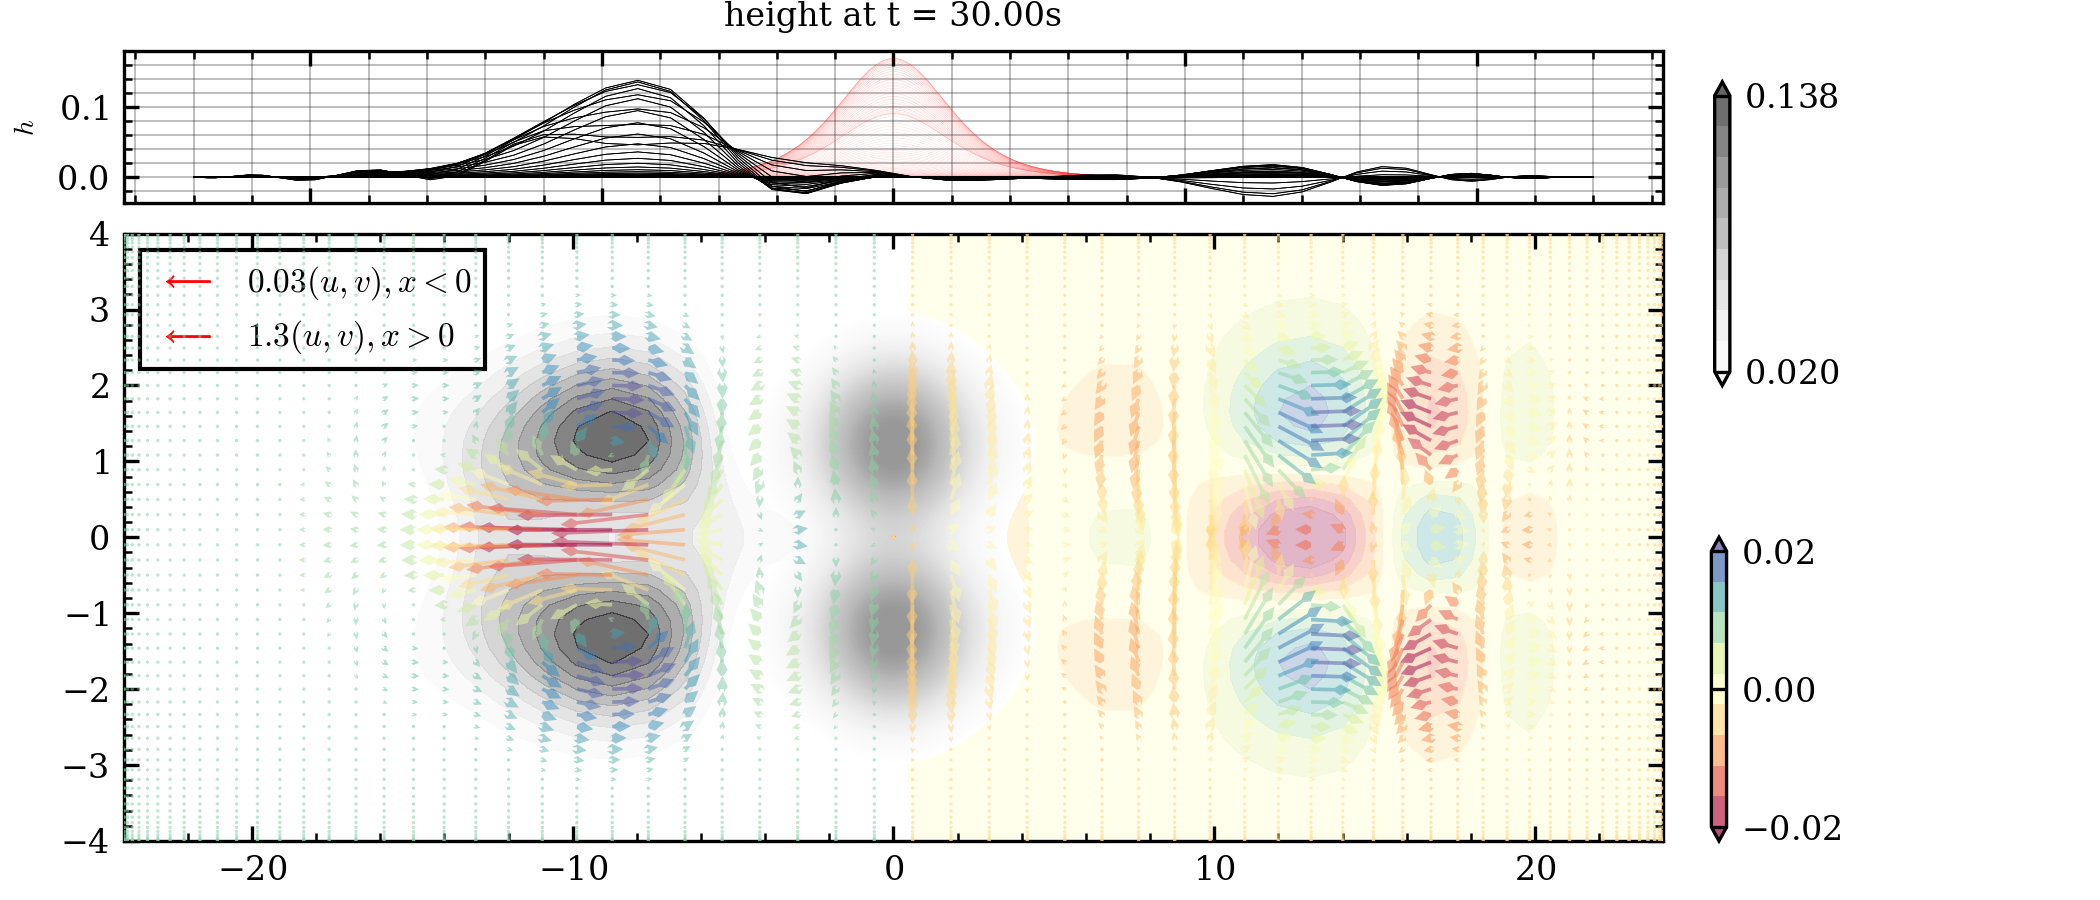
\includegraphics[width=\textwidth]{./figure/soliton.png}
    \end{figure}
    \begin{itemize}
        \item westward propagation of the soliton
        \item strongly dispersive instabilities
        \item periodic shedding
        \item one can show that these instabilities are barotropic modes
    \end{itemize}
\end{frame}
\subsubsection{Mass and energy conservation}
\begin{frame}
    \frametitle{Mass and energy conservation}
    \begin{minipage}{.7\linewidth}
        \begin{figure}[H]
            \centering
            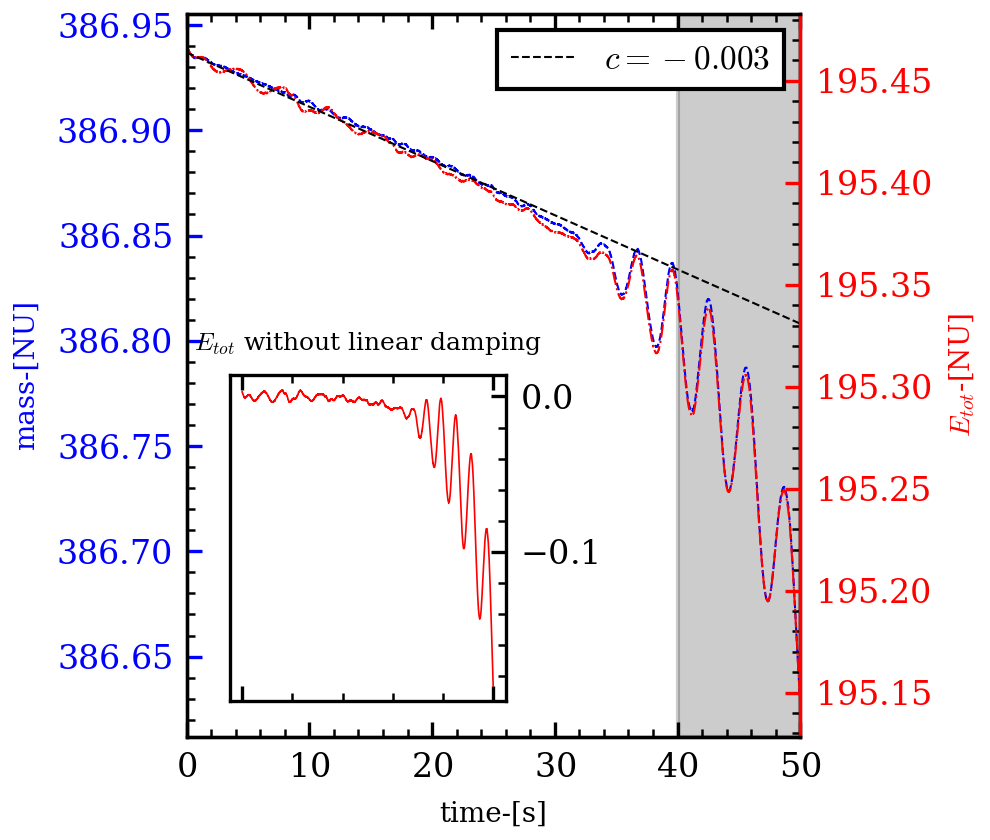
\includegraphics[width=\linewidth]{./figure/energy.png}
        \end{figure}
    \end{minipage}
    \begin{minipage}{.28\linewidth}
        \begin{itemize}
            \item quite good conservation ($\sim e^{-4}$)
            \item linear numerical damping
            \item sponge layer to avoid effect of Boundaries
        \end{itemize}
    \end{minipage}
\end{frame}
\subsubsection{Potential Enstrophy}
\begin{frame}
    \frametitle{Enstrophy Conservation}
    \begin{minipage}{.6\linewidth}

        \begin{figure}[H]
            \centering
            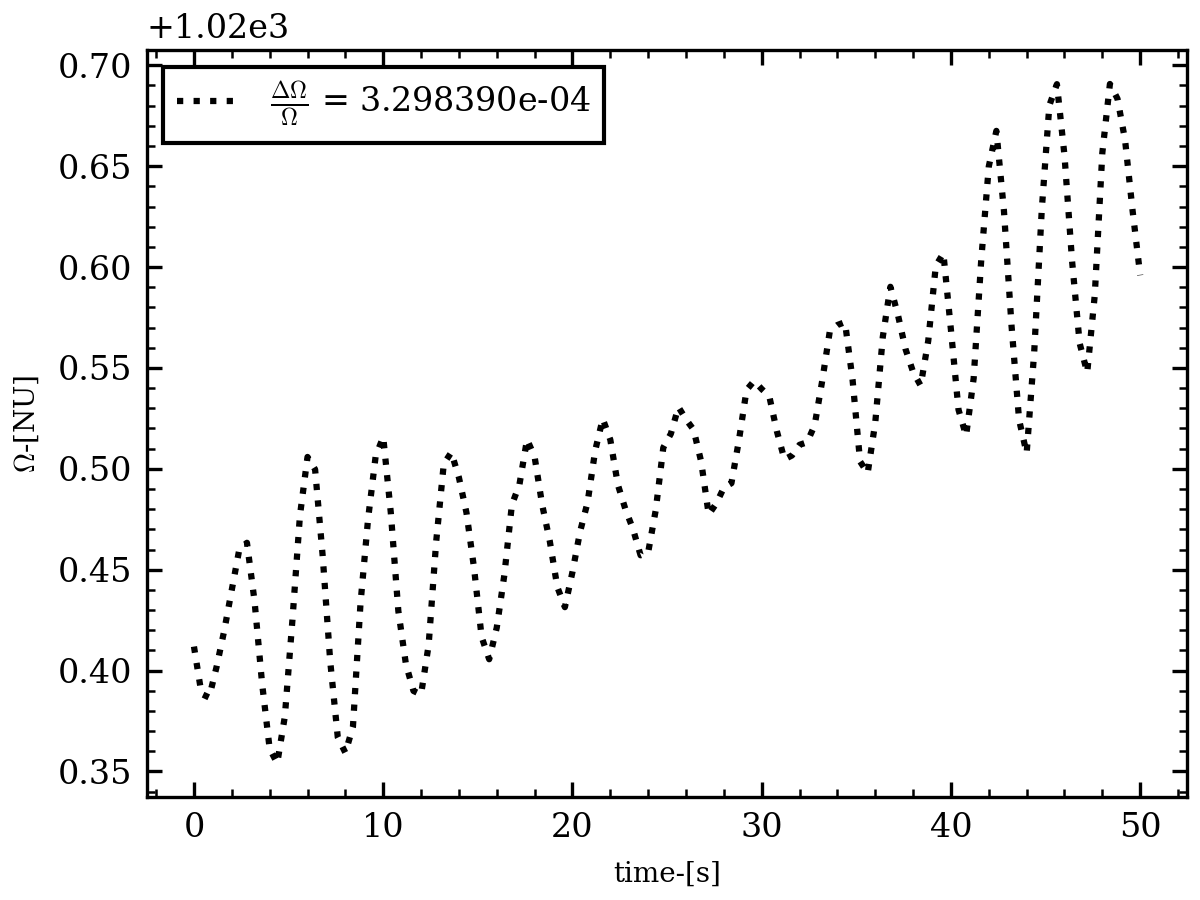
\includegraphics[width=\linewidth]{./figure/potential_enstrophy.png}
        \end{figure}
    \end{minipage}
    \begin{minipage}{.38\linewidth}

        \begin{itemize}
            \item Conservative value
            \item radiative instabilities have great impact in the $v$-field
            \item radiative shed are antisymmetric parts of the wave
            \item oscillations are caused by successive radiations
            \item constant increasing die to shedding
        \end{itemize}
    \end{minipage}
\end{frame}
\subsubsection{Phase speed evaluation}
\begin{frame}
    \frametitle{Phase speed evaluation}
    \begin{minipage}{.6\linewidth}

        \begin{figure}[H]
            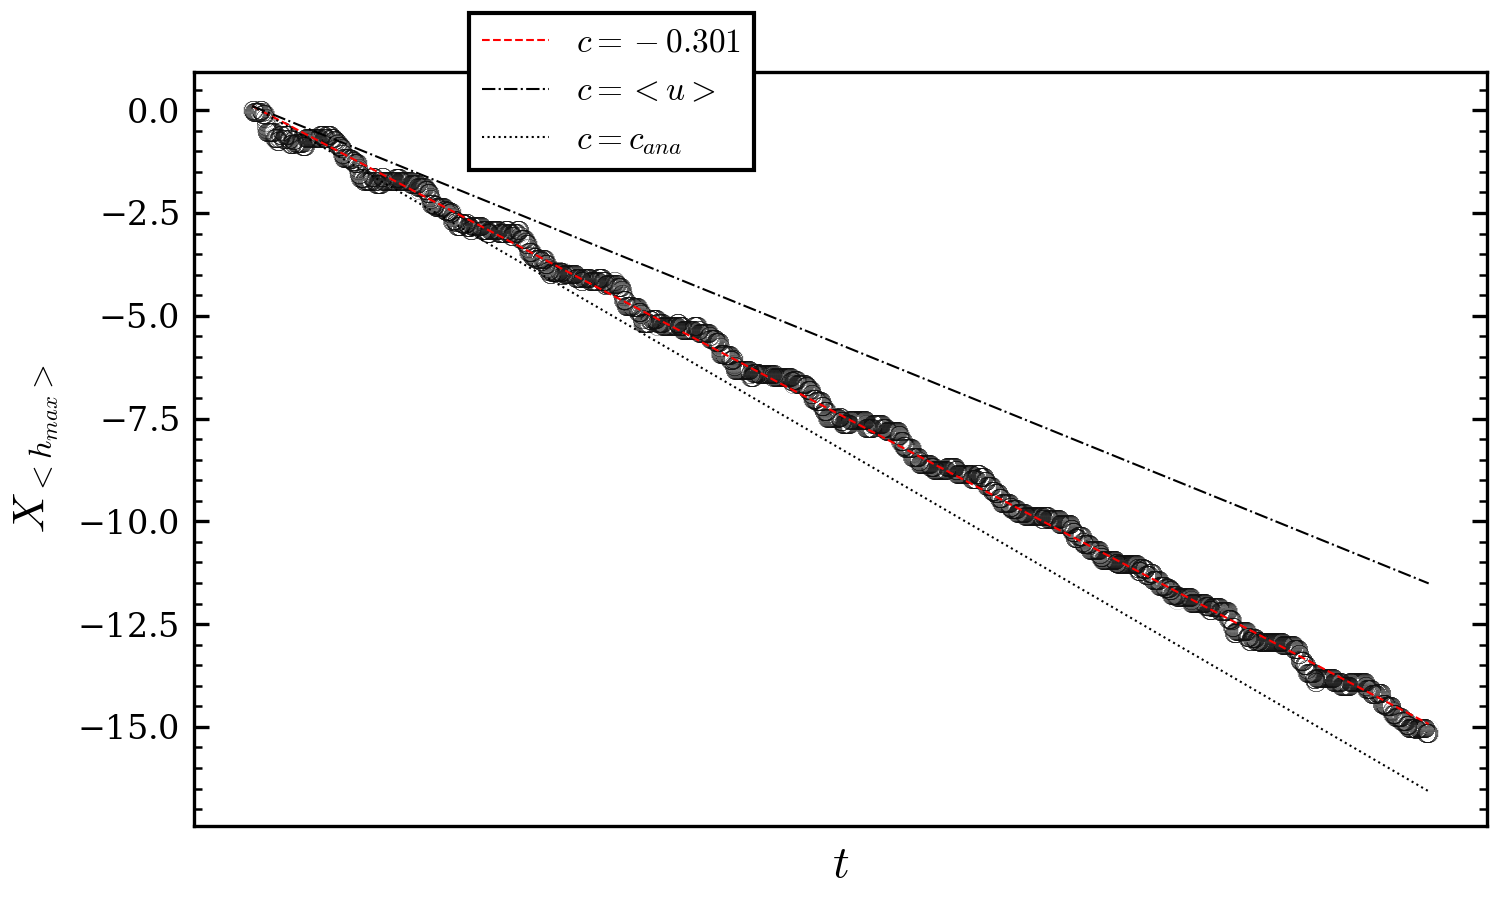
\includegraphics[width=\linewidth]{./figure/mean_height.png}
            \caption{Phase speeds evaluation}
        \end{figure}
    \end{minipage}
    \begin{minipage}{.3\linewidth}
        \begin{itemize}
            \item Position of a maximum window during time
            \item $c_\Phi = -0.301$
            \item close to the $\frac{1}{3}$ theoretical one
        \end{itemize}
    \end{minipage}

\end{frame}

\subsection{Kelvin soliton waves}
\begin{frame}
    \frametitle{Kelvin wave}
    Following wave satisfying the Kelvin equation
    \begin{equation}
        \label{eq:Kelvin wave}
        \begin{cases}
            h(x,y,t = 0) = H_0  \frac{\sigma}{k} \exp(- ((kx) ^2 +(ly)^ 2)) \\
            u(x.y, t = 0) = H_0 \exp(- ((kx) ^2 +(ly)^ 2))                  \\
            v(x,y,t=0) = 0
        \end{cases}
    \end{equation}
\end{frame}
\begin{frame}
    \frametitle{Kelvin wave}
    \begin{figure}[H]
        \centering
        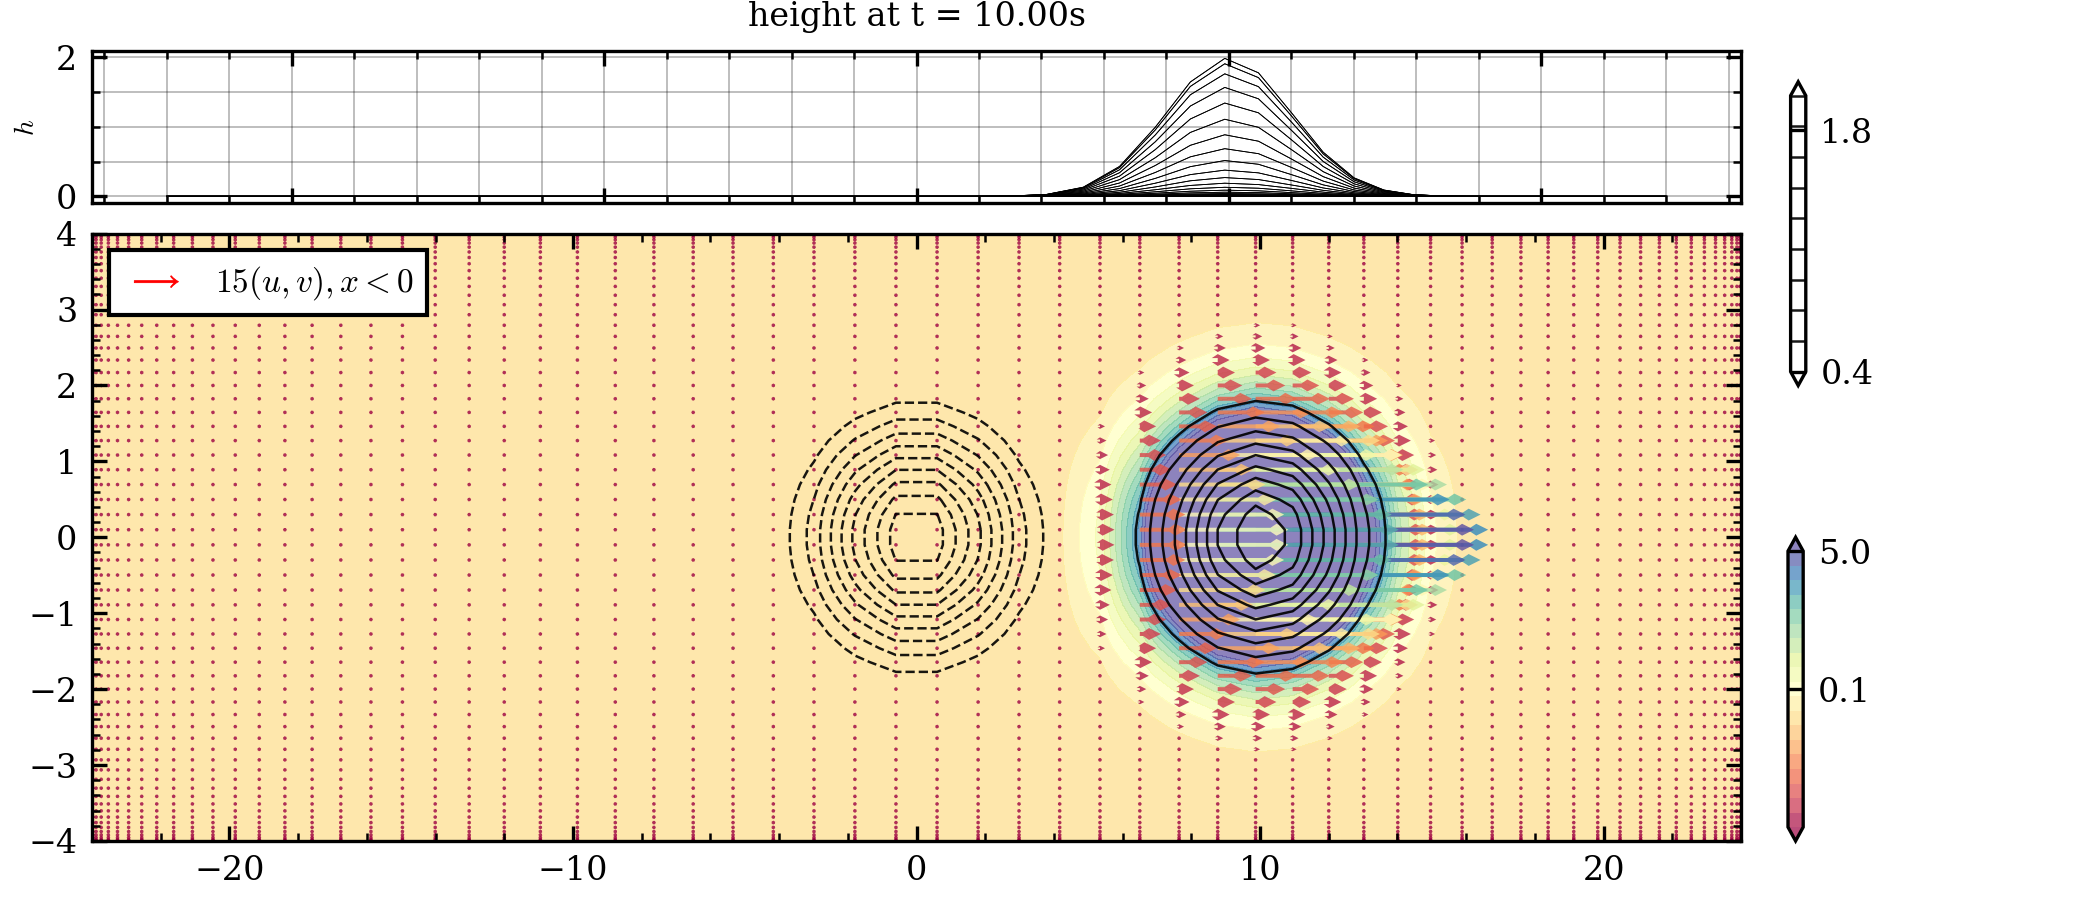
\includegraphics[width=\textwidth]{./figure/kelvin_wave.png}
    \end{figure}
    \begin{itemize}
        \item eastward propagation of the wave
        \item faster than Rossby waves
        \item no dispersion
        \item no north-south velocity field
    \end{itemize}
\end{frame}
\subsubsection{Mass and energy conservation}
\begin{frame}
    \frametitle{Energy and mass conservation}
    \begin{minipage}{.7\linewidth}
        \begin{figure}[H]
            \centering
            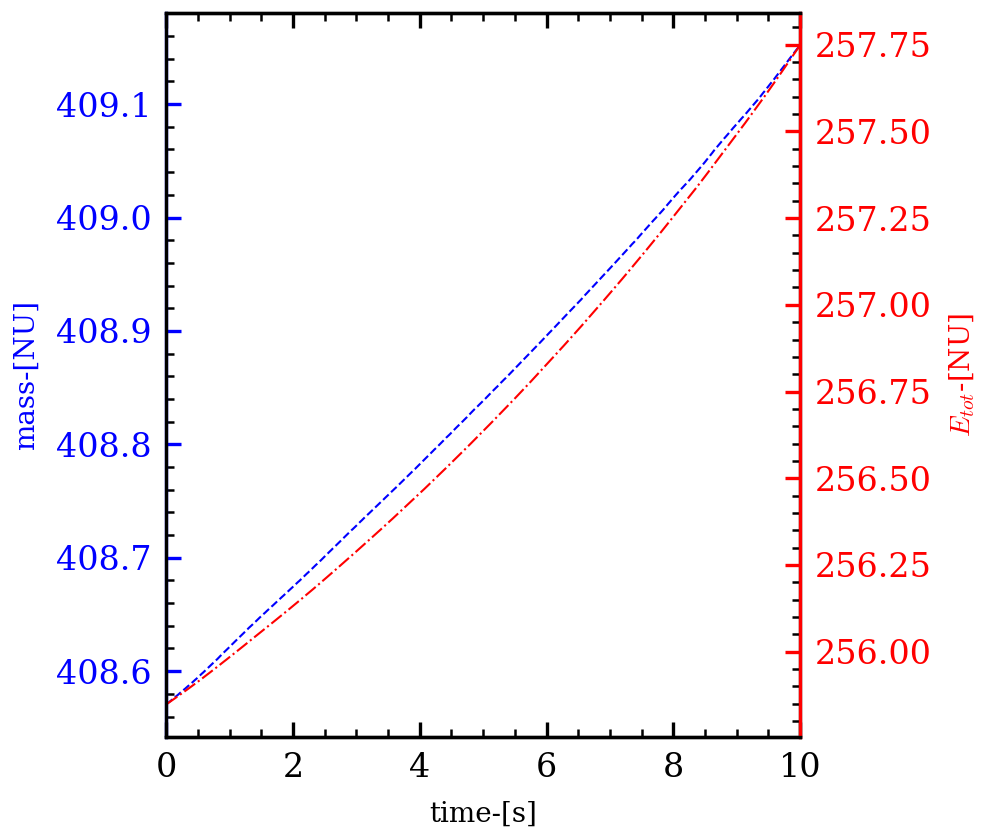
\includegraphics[width=\linewidth]{./figure/energy_kelvin_wave.png}
        \end{figure}
    \end{minipage}
    \begin{minipage}{.28\linewidth}
        \begin{itemize}
            \item quite conservation : relative conservation of $\sim e^{-3}$
            \item relative error greater than for Rossby waves (CFL condition)
        \end{itemize}
    \end{minipage}
\end{frame}
\subsubsection{Potential Enstrophy}
\begin{frame}
    \frametitle{Enstrophy Conservation}
    \begin{minipage}{.6\linewidth}

        \begin{figure}[H]
            \centering
            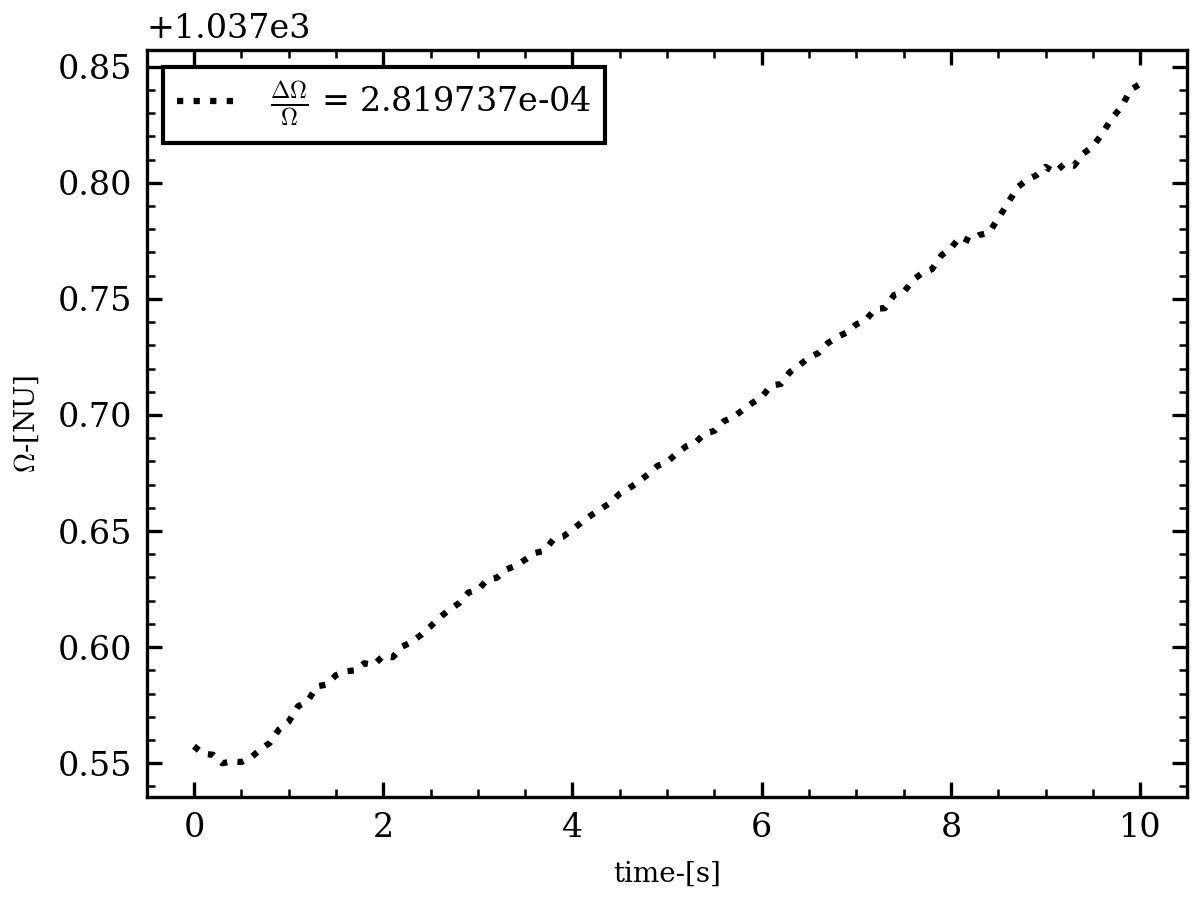
\includegraphics[width=1\linewidth]{./figure/potential_enstrophy_kelvin_wave.png}
        \end{figure}
    \end{minipage}
    \begin{minipage}{.38\linewidth}

        \begin{itemize}
            \item quite constant ($2e^{-4}$)
            \item no oscillations : no instabilities

        \end{itemize}
    \end{minipage}
\end{frame}
\subsubsection{Phase speed evaluation \& dispersion}
\begin{frame}
    \frametitle{Phase velocity \& dispersion}
    \begin{minipage}{.6\linewidth}

        \begin{figure}[H]
            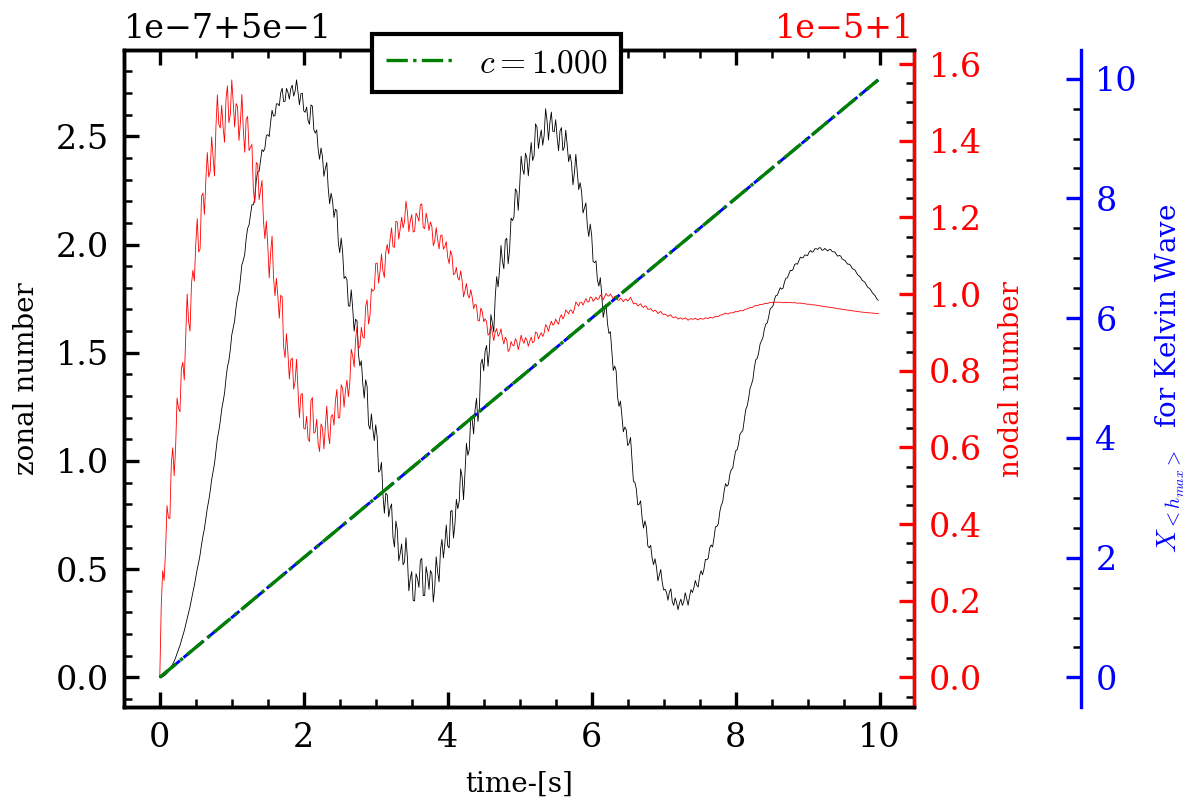
\includegraphics[width=\linewidth]{./figure/kelvin_wave_param.png}
            \caption{Phase speed and dispersion evaluation}
        \end{figure}
    \end{minipage}
    \begin{minipage}{.3\linewidth}
        \begin{itemize}
            \item Fit of the kelvin wave by an original Kelvin wave
            \item $c_\Phi = 1.000 = c_{ana}$
            \item relative dispersion of $1e^{-5}$
        \end{itemize}
    \end{minipage}
\end{frame}

\subsection{Unstable waves}
\begin{frame}
    \frametitle{Unstable wave study}
    Kelvin like wave shape, with velocity, gravity spreading.
    \begin{equation}
        \label{eq:sharp wave}
        \begin{cases}
            h(x,y,t = 0) = H_0  \exp(- ((0.5x) ^2 +(y)^ 2)) \\
            u(x.y, t = 0) = 0                               \\
            v(x,y,t=0) = 0
        \end{cases}
    \end{equation}
    Note that as the gravity is the only force applied at the beginning, the wave should spread equally in every direction, hence the \textbf{mass of fluid should be equally distributed} east-west.

\end{frame}
\begin{frame}
    \frametitle{Unstable wave study}
    \begin{figure}[H]
        \centering
        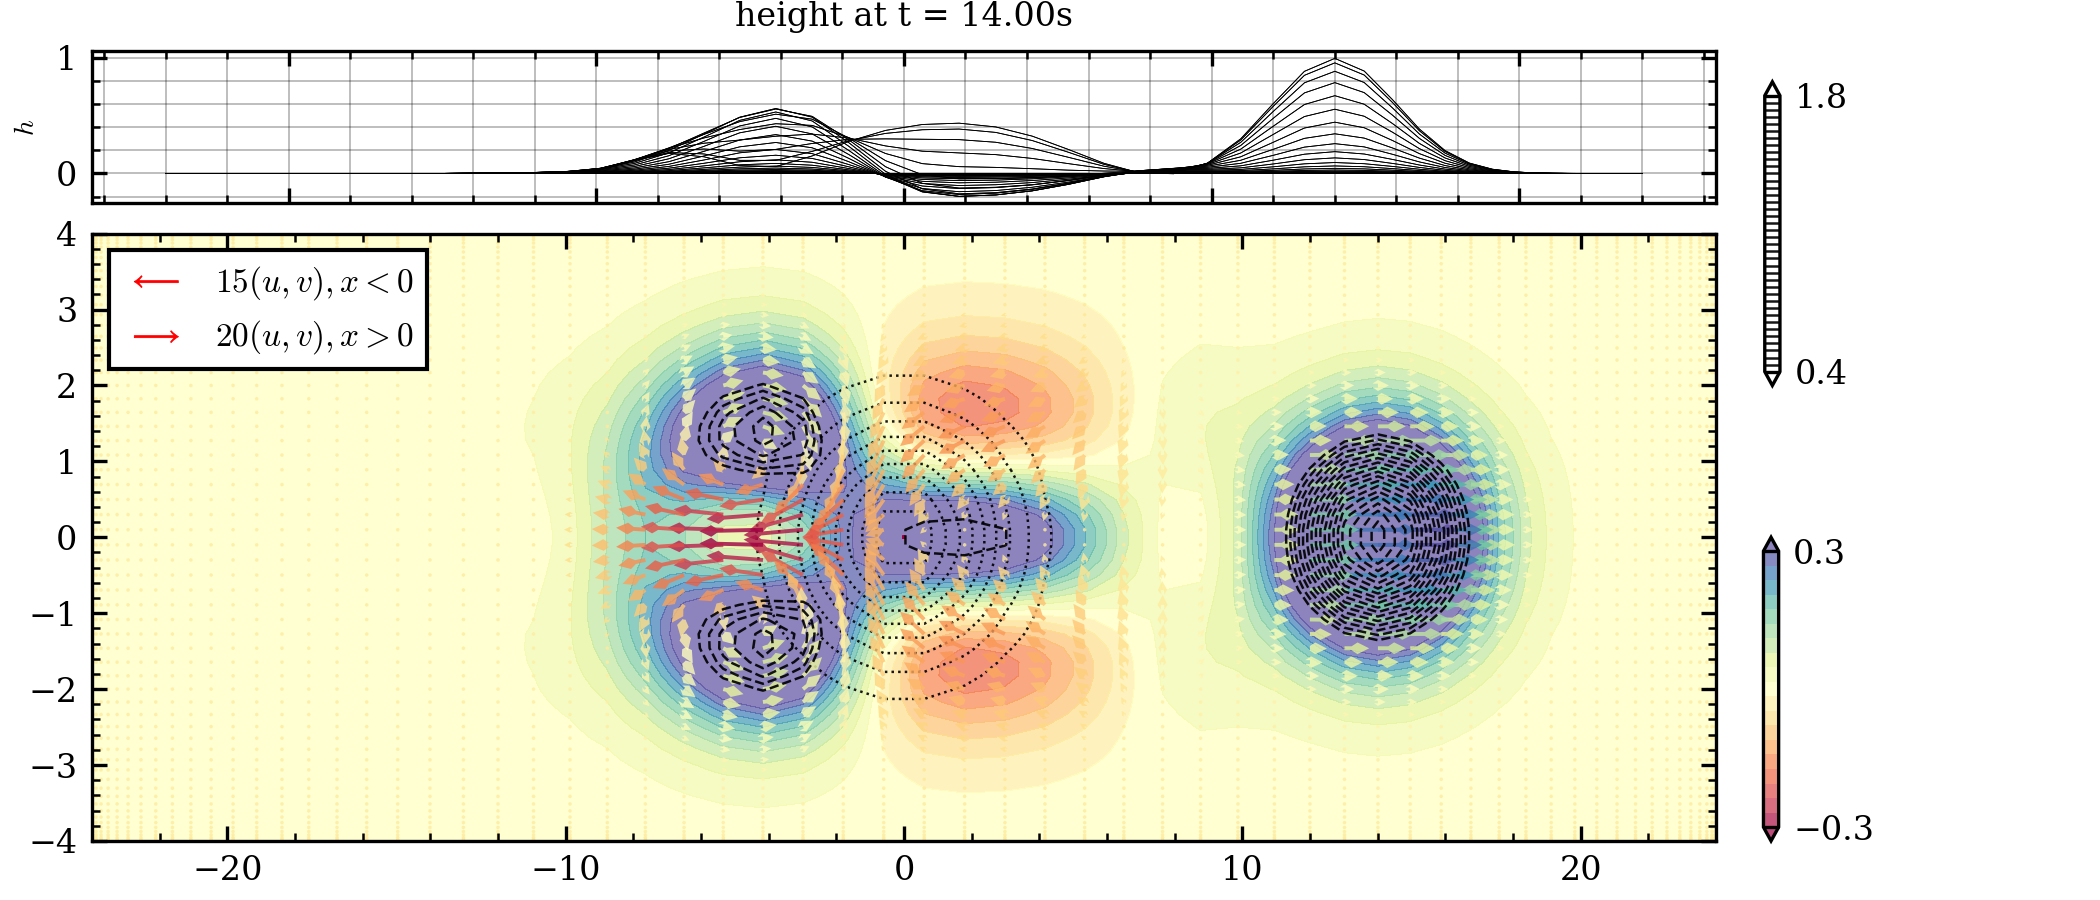
\includegraphics[width=\textwidth]{./figure/kelvin_wave_0_speed.png}
    \end{figure}
    \begin{itemize}
        \item Rossby soliton $n = 1$ westard
        \item Kelvin wave eastward
        \item Radiative instabilities
        \item energy repartition between modes
    \end{itemize}
\end{frame}
\subsubsection{Mass and energy conservation}
\begin{frame}
    \frametitle{Energy repartition between mode}
    \begin{minipage}{.4\linewidth}
        \begin{figure}[H]
            \centering
            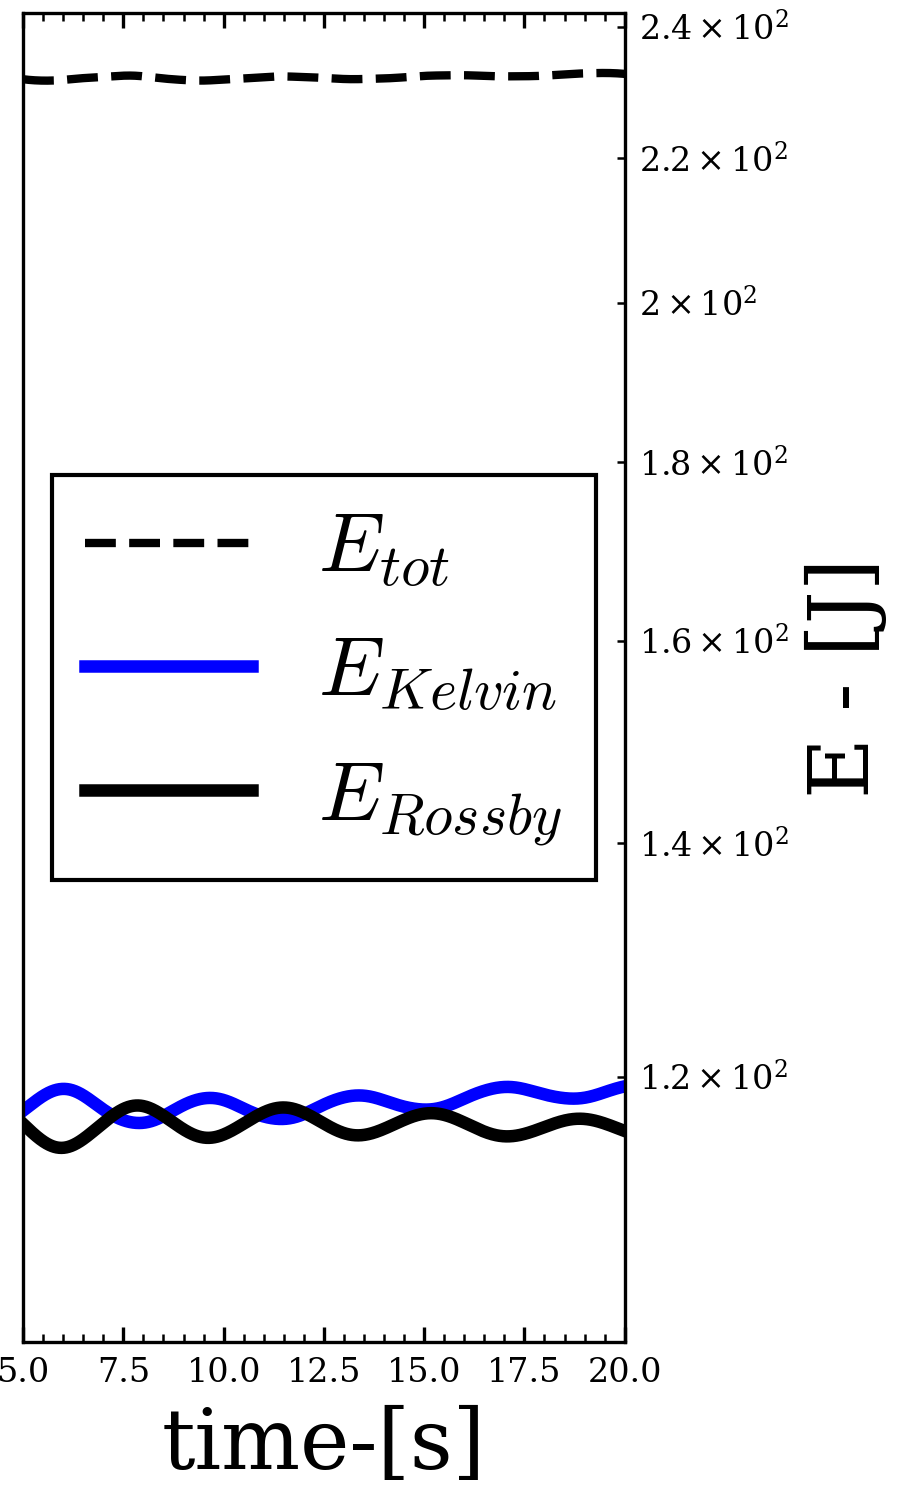
\includegraphics[width=1\linewidth]{./figure/energy_repartition.png}
        \end{figure}
    \end{minipage}
    \begin{minipage}{.58\linewidth}
        \begin{itemize}
            \item $V_{\text{Kelvin}} = 2 \pi H_0 kl$
            \item 2 times smaller than the initial unstable wave
            \item equally distributed Mass, but Kelvin wave is 3 times faster
            \item $T_{\text{Kelvin}} = 9 T_{\text{Rossby}}$.
            \item $\pi / 2$ phase shifted
        \end{itemize}
    \end{minipage}
\end{frame}

\begin{frame}
    \frametitle{Mass and Energy conservation}
    \begin{minipage}{.7\linewidth}
        \begin{figure}[H]
            \centering
            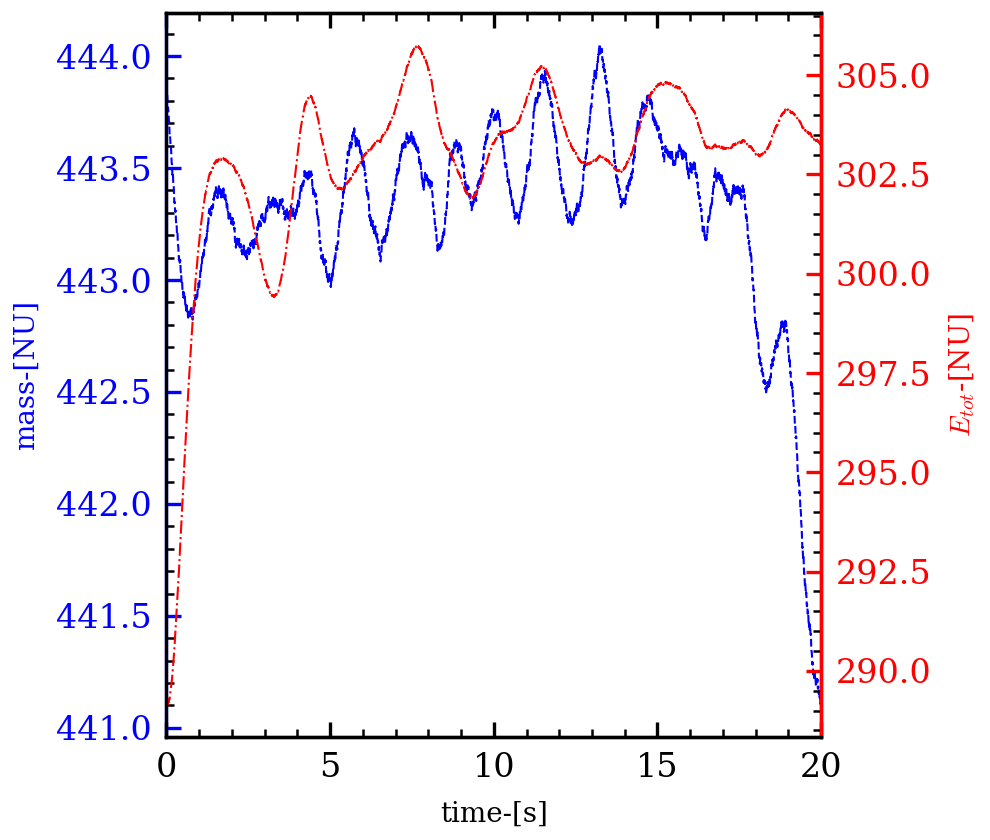
\includegraphics[width=\linewidth]{./figure/energy_common_wave.png}
        \end{figure}
    \end{minipage}
    \begin{minipage}{.28\linewidth}
        \begin{itemize}
            \item quite conservation : relative conservation of $6\sim e^{-3}$
            \item no dissipation (Rossby decrease, Kelvin increase)
            \item oscillations correlated with instabilities shed
        \end{itemize}
    \end{minipage}
\end{frame}
\subsubsection{Potential Enstrophy}
\begin{frame}
    \frametitle{Enstrophy Conservation}
    \begin{minipage}{.6\linewidth}

        \begin{figure}[H]
            \centering
            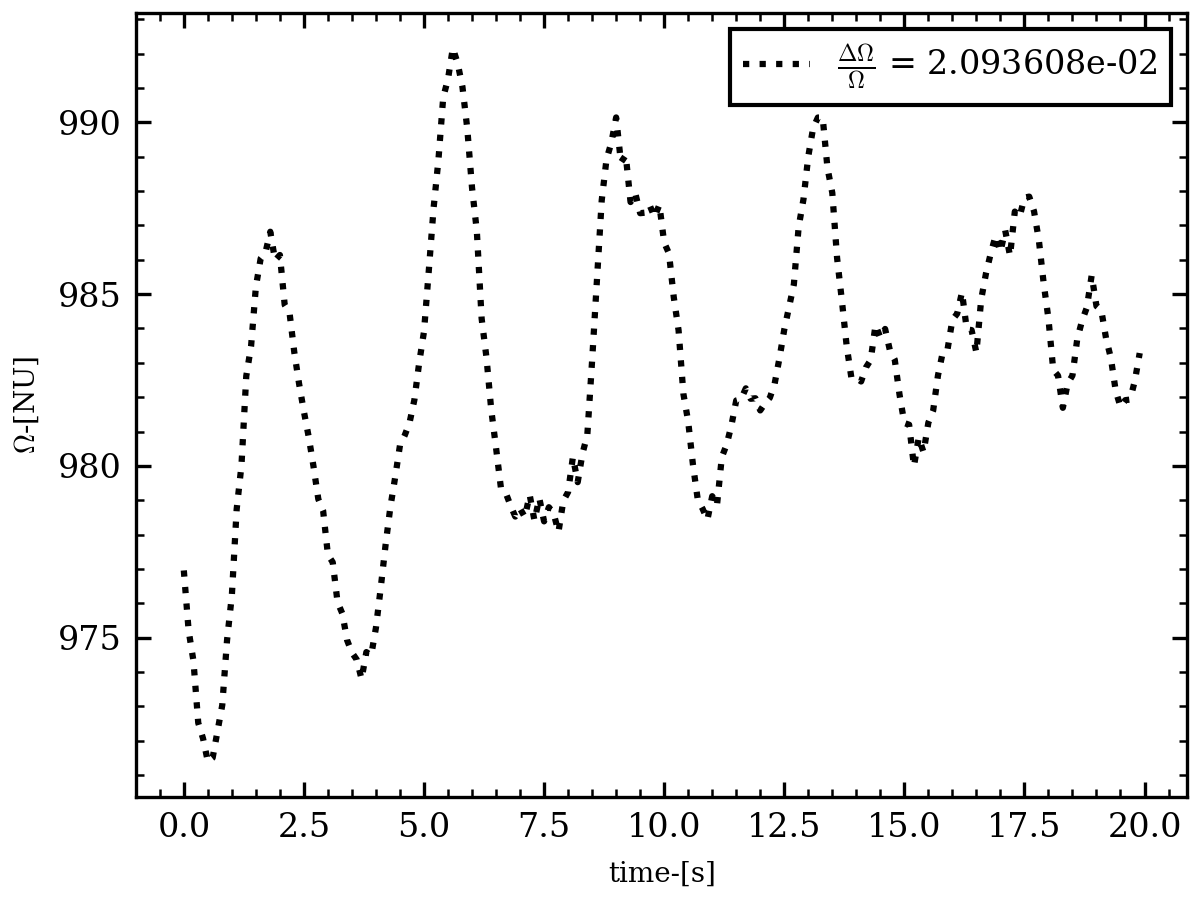
\includegraphics[width=1\linewidth]{./figure/potential_enstrophy_common_wave.png}
        \end{figure}
    \end{minipage}
    \begin{minipage}{.38\linewidth}

        \begin{itemize}
            \item high relative value $2e^-2$
            \item CLF and instabilities

        \end{itemize}
    \end{minipage}
\end{frame}
\subsubsection{Phase speed evaluation \& dispersion}
\begin{frame}
    \frametitle{Phase speed \& dispersion}
    \begin{minipage}{.6\linewidth}

        \begin{figure}[H]
            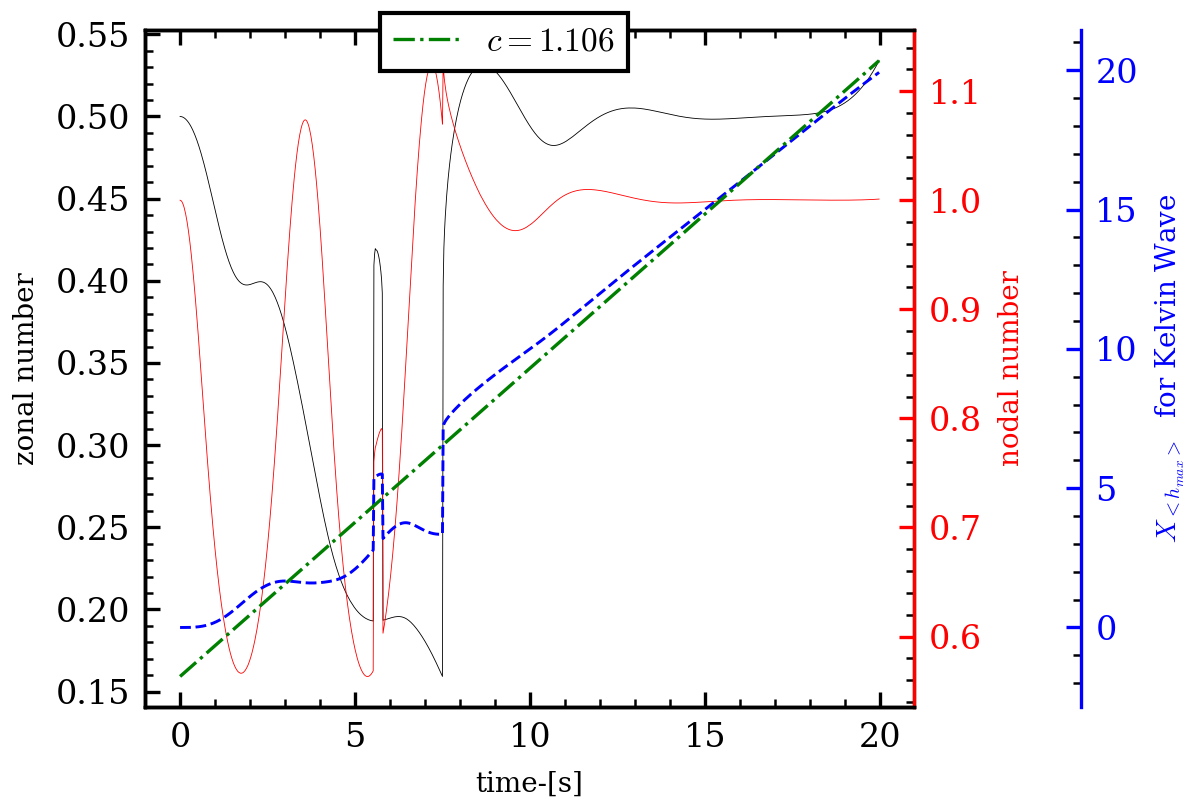
\includegraphics[width=1\linewidth]{./figure/0velocity_wave_params.png}
            \caption{Phase speed and dispersion evaluation of Kelvin Wave}
        \end{figure}
    \end{minipage}
    \begin{minipage}{.3\linewidth}
        \begin{itemize}
            \item Only the height of the wave has changed
            \item $c_\Phi = 1.106$
            \item no dispersion at high t (zonal and nodal wave number constant)
        \end{itemize}
    \end{minipage}
\end{frame}

\begin{frame}
    \frametitle{Phase speed \& dispersion}
    \begin{minipage}{.6\linewidth}
        \begin{figure}[H]
            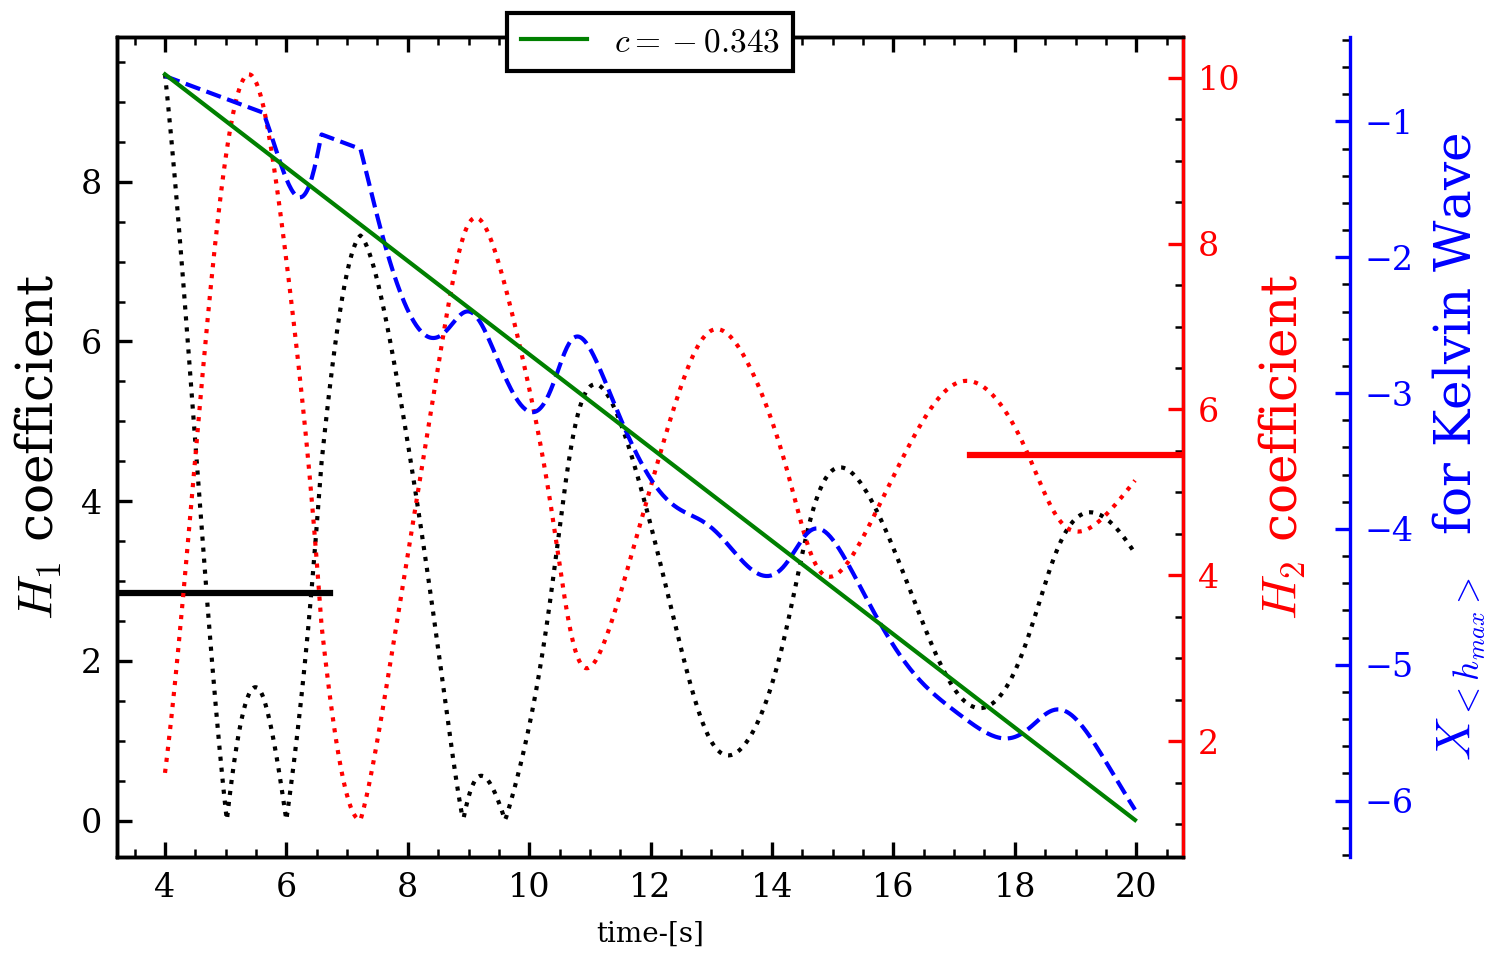
\includegraphics[width=1\linewidth]{./figure/0velocity_wave_params_rossby.png}
            \caption{Phase speed and dispersion evaluation of Rossby Wave}
        \end{figure}
    \end{minipage}
    \begin{minipage}{.3\linewidth}
        \begin{itemize}
            \item $c_\Phi = -0.304$
            \item Hermite coefficient oscillating around a steady state
            \item stands for variation in the ratio : $\frac{k}{\sigma}$, when instabilities are shed
        \end{itemize}
    \end{minipage}
\end{frame}

\begin{frame}
    \frametitle{Conclusion}
    \begin{itemize}
        \item Chebyshev and 2 order integration scheme
        \item Analyses on 3 different types of wave
        \item Study of modes of propagation
        \item Using mass, energy and enstrophy conservation
        \item Study of dissipation and propagation speed of the wave
    \end{itemize}
\end{frame}
\section{Conclusion}
\begin{frame}
    \frametitle{Perspective}
    \begin{itemize}
        \item Study of sponge layer to avoid influence of boundary
        \item Study of higher modes, and their repartition in energy

    \end{itemize}
\end{frame}

\end{document}